\documentclass{article}
\usepackage{imakeidx} % Per creare un vero indice
%\usepackage{tcolorbox}
\usepackage{xcolor}
\usepackage[utf8]{inputenc}
\usepackage[T1]{fontenc}
\usepackage[italian]{babel}
\usepackage{multicol}
\usepackage{makecell}
\usepackage{pdfpages}
\usepackage{geometry}
\usepackage{array}
\usepackage{multirow, tabularx}
\usepackage{float}
\usepackage{colortbl}
\usepackage{graphicx} % Per l'inserimento di immagini

\def\arraystretch{1.5}
\renewcommand\theadalign{bc}
\renewcommand\theadfont{\bfseries}
\renewcommand\theadgape{\Gape[4pt]}
\newcolumntype{Y}{>{\centering\arraybackslash}X}

\makeindex
\definecolor{dark_purple}{RGB}{48, 25, 52}

\begin{document}
	\begin{center}
		\textbf{UNIVERSITÀ DEGLI STUDI DI NAPOLI \\ FEDERICO II}
		\\
		\vspace{1cm}
		
\includegraphics[width=0.2\textwidth]{logo_universita.png} 
	\end{center}
	
	\vspace{1cm}
	
	\begin{center}
		\textbf{Corso di Ingegneria del Software} \\
		\vspace{0.5cm}
		\textbf{DIPARTIMENTO DI INGEGNERIA ELETTRICA E TECNOLOGIE DELL'INFORMAZIONE} \\
		\vspace{0.5cm}
		
\includegraphics[width=0.6\textwidth]{logo_sfondo} \\
		\textbf{\textcolor{dark_purple}{Enjoy music, enjoy the lab}}
		
	\end{center}
	
	\vspace{0.5cm}
	
	\begin{center}
		\textbf{Candidati:} \\
		Fabrizio Di Giovanni - N8600- \\
		Lucia Brando - N86003382 \\
		Dario Morace - N8600- \\
		ID GRUPPO:- - - - -\\
	\end{center}
	
	\vspace{0.5cm}
	
	\begin{center}
		\textbf{Docenti:} \\
		Prof. Sergio Di Martino \\
		Prof. Francesco Cutugno
	\end{center}
	
	\vspace{0.5cm}
	
	\begin{center}
		\textbf{ANNO ACCADEMICO 2023/2024}
	\end{center}
	

	\renewcommand{\contentsname}{Indice} % Rinomina la tabella dei contenuti
	\tableofcontents % Genera la tabella dei contenuti
	
	\clearpage
	
	\section{Introduzione}
	Si vuole realizzare, dietro commissione della società SoftEngUniNA, una piattaforma per gli appassionati di musica
	Nello specifico, la società ha richiesto la progettazione e implementazione di un applicativo mobile, oltre alla parziale verifica dei moduli necessari per il suo corretto funzionamento.
	Nasce così \textbf{\textit{\textcolor{dark_purple}{SoundLab}}}, un nuovo spazio dedicato a tutti coloro che fanno della musica la colonna portante delle loro giornate.
		\subsection{Che cos'è SoundLab}
		SoundLab è un servizio dedicato agli appassionati di musica, offrendo una vasta selezione di brani e generi musicali per soddisfare i gusti di tutti gli utenti registrati. Gli utenti possono accedere al sistema per esplorare e ascoltare musica, creare e gestire le proprie playlist, visibili sui loro profili personali. \\Inoltre, gli amministratori hanno accesso a strumenti di analisi avanzati, permettendo loro di visualizzare le statistiche relative ai brani e agli utenti presenti nel sistema, migliorando così l'esperienza complessiva degli utenti.
		\\
		\begin{figure}[h]
			\centering
			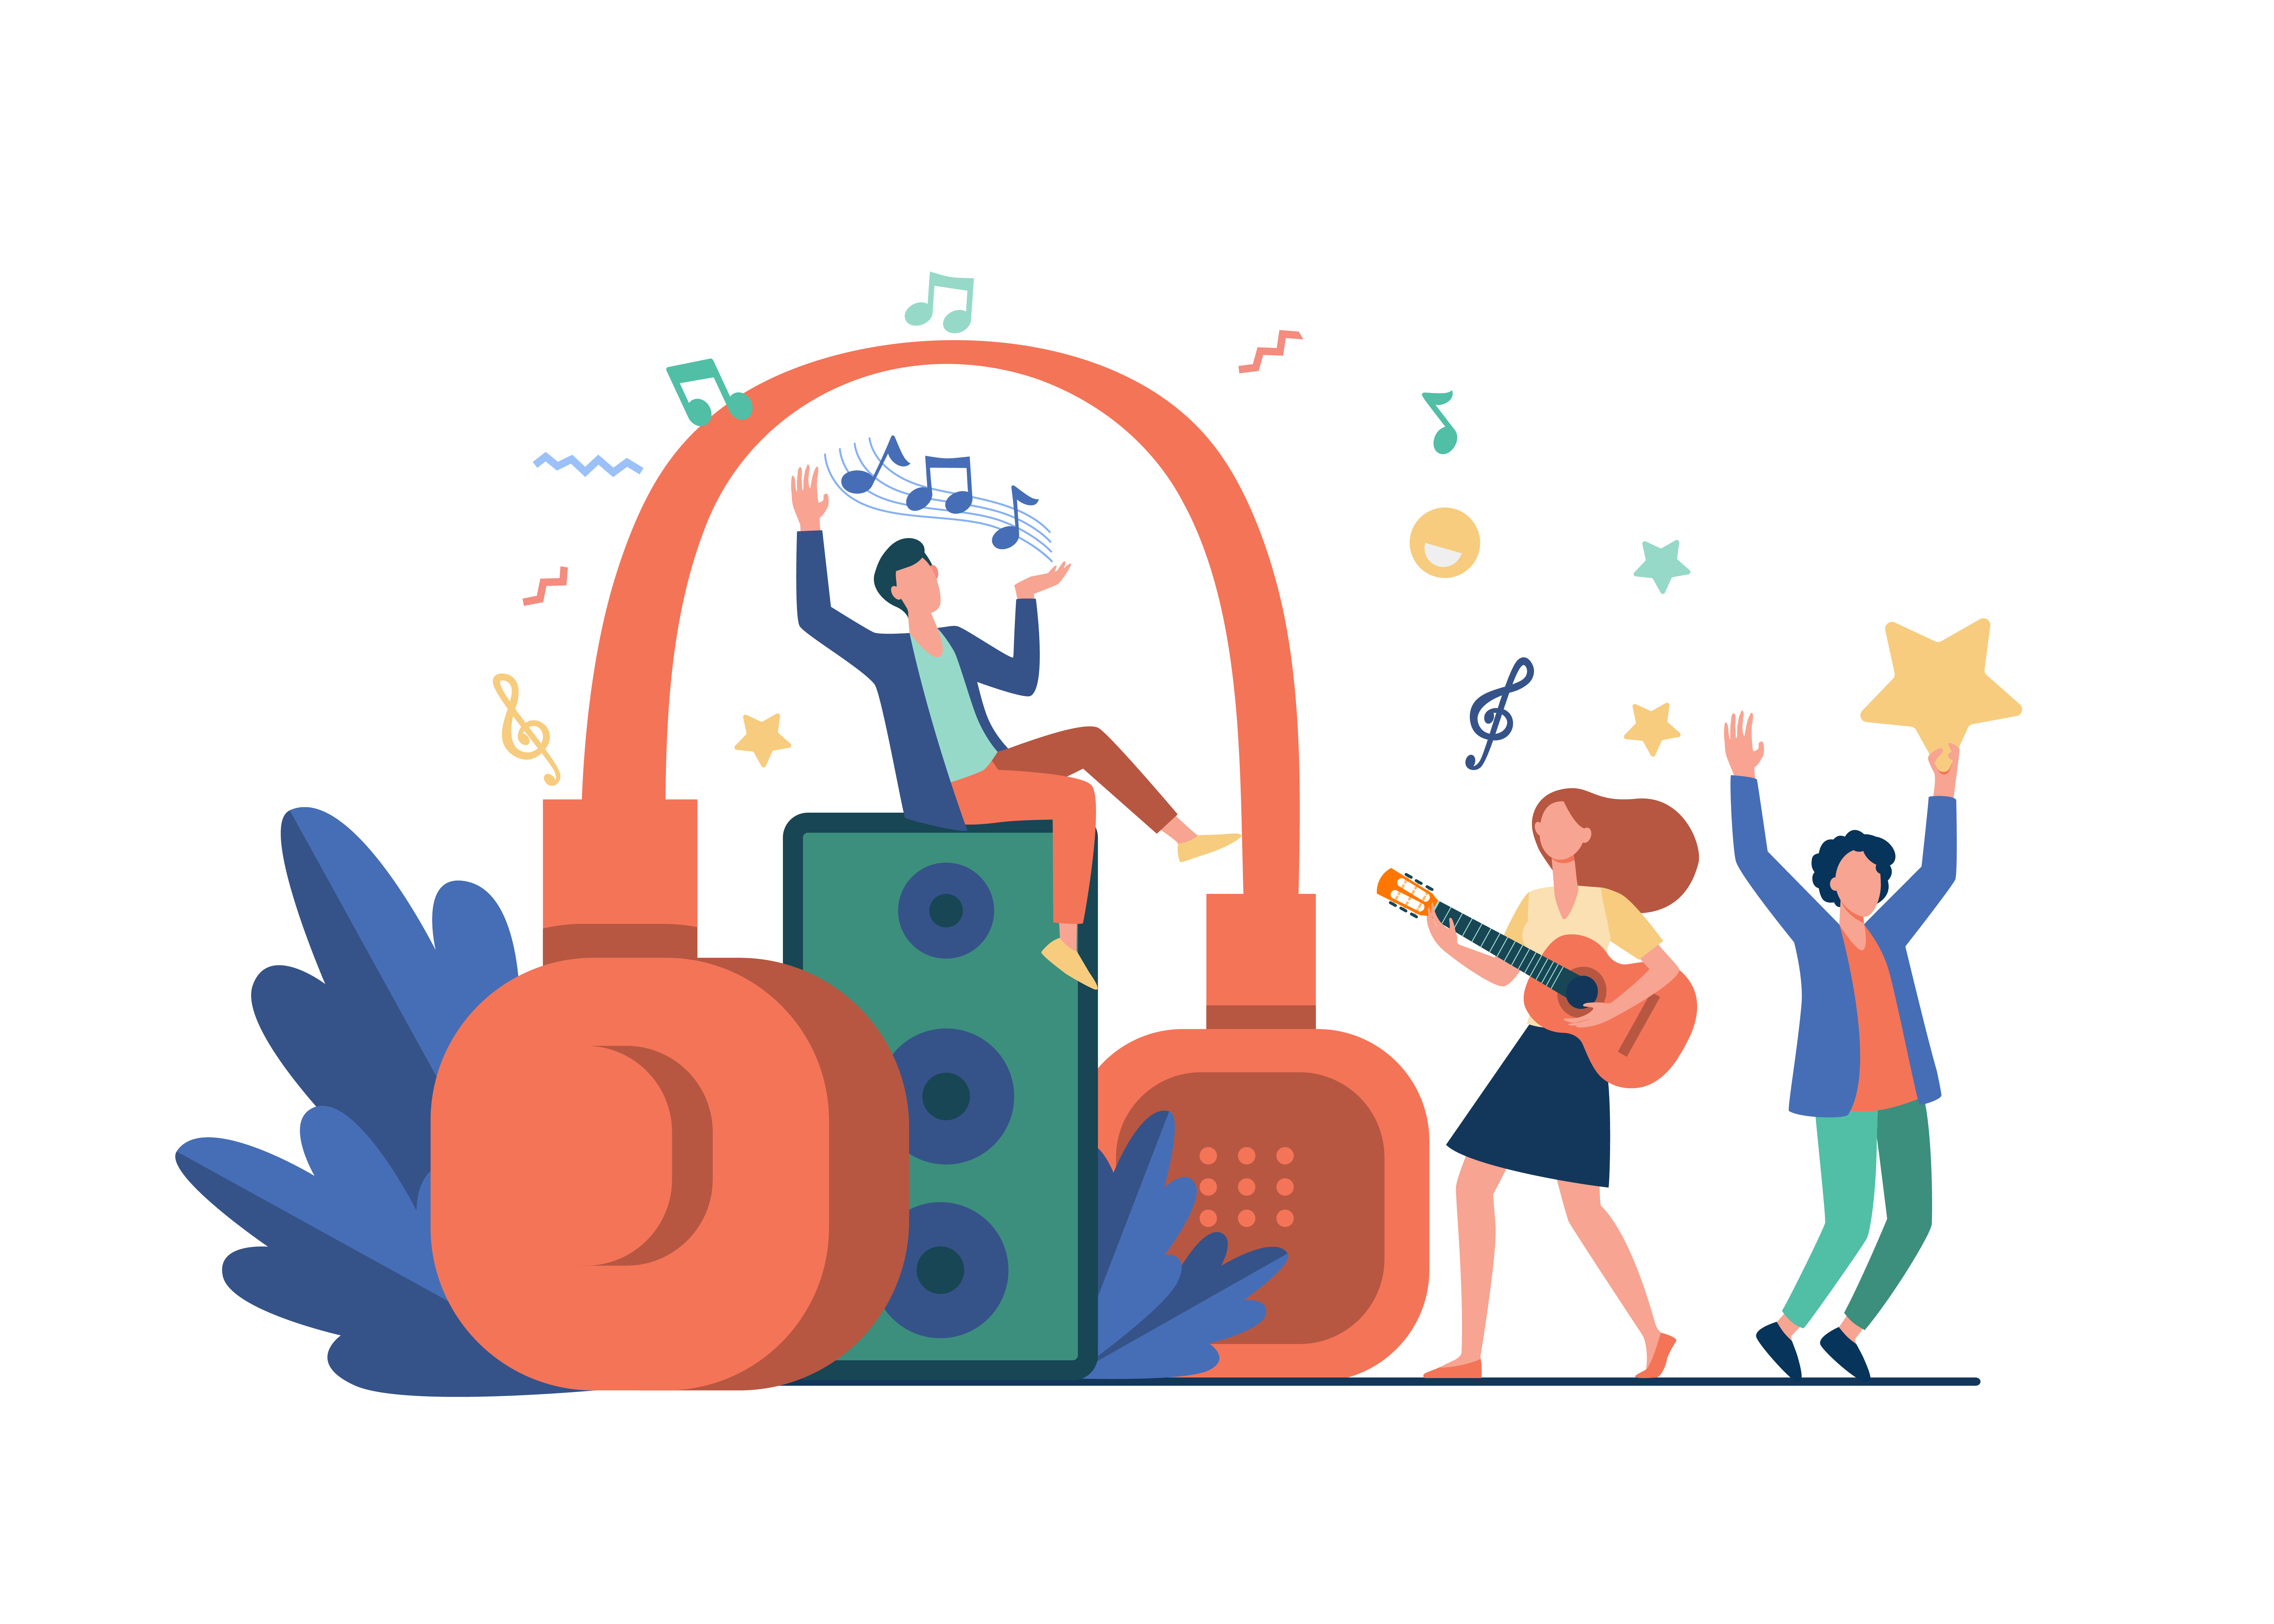
\includegraphics[width=0.9\textwidth]{/Users/lucia/Desktop/INGSW/documentazioni/5870}
			\label{fig:first_pic}
		\end{figure}
		\\
		In conformità con i recenti standard previsti dall’Unione Europea, Soundlab si impegna all’assoluto rispetto della privacy e dei dati della propria utenza per assicurare un’esperienza di navigazione sicura; proprio perché abbiamo a cuore tale sicurezza, il nostro staff si impegna a offre un’assistenza a 360 gradi.
		\subsection{Cosa offre Soundlab}
		Per offrire un'esperienza ottimale, SoundLab si basa su un robusto \textbf{\textit{\textcolor{dark_purple}{back-end}}} progettato per garantire prestazioni elevate e scalabilità in base alle esigenze dell'utenza. Questo sistema back-end avanzato assicura che l'applicazione possa gestire efficacemente un numero crescente di utenti e richieste, mantenendo sempre una risposta rapida e affidabile.\\
		Dall'altro lato, Soundlab presenta un'interfaccia \textbf{\textit{\textcolor{dark_purple}{front-end}}} semplice e moderna, progettata per rendere intuitiva la navigazione. Gli utenti possono facilmente cercare, esplorare e interagire con contenuti e funzionalità dell'applicazione, rendendo la loro esperienza unica e adattabile alle loro preferenze personali.\\ 
		La combinazione di un back-end potente e un'interfaccia utente intuitiva permette a SoundLab di offrire un servizio eccezionale, migliorando la soddisfazione degli utenti e favorendo un'interazione più profonda con la piattaforma.
		\subsection{Tecnologie utilizzate}
		L'applicativo è sviluppato interamente su piattaforma \textbf{\textit{\textcolor{dark_purple}{Android}}} utilizzando il linguaggio di programmazione \textbf{\textit{\textcolor{dark_purple}{Object-Oriented}}}, in particolare \textbf{\textit{\textcolor{dark_purple}{Java}}}.\\
		Questa scelta tecnologica garantisce robustezza, flessibilità e una vasta compatibilità con dispositivi Android di diverse generazioni. Inoltre, l'applicazione è dotata di un sistema di logging avanzato che facilita il testing efficace e la risoluzione rapida dei problemi, migliorando la qualità complessiva del software e l'esperienza utente.\\
		Per il back-end, SoundLab sfrutta tecnologie all'avanguardia, tra cui servizi di \textit{public Cloud Computing} come (???), che permettono di massimizzare la scalabilità e le prestazioni del sistema. Questi servizi cloud offrono una piattaforma affidabile e sicura per la gestione dei dati, consentendo al sistema di adattarsi dinamicamente al crescente numero di utenti e alle richieste variabili. La combinazione di un'applicazione front-end potente e intuitiva con un back-end scalabile e performante garantisce un servizio eccellente e un'esperienza utente ottimale.
		\\
		\\
		Nei capitoli successivi, approfondiremo ulteriormente il discorso sulle tecnologie utilizzate e forniremo, come richiesto da SoftEngUniNa, i documenti relativi al lavoro svolto per la realizzazione del progetto.
	\section{Modello Funzionale}
	In questa sezione andremo a descrivere il modello funzionale del software partendo da un'analisi dei casi d'uso assegnati per l'applicativo.
		\subsection{Requisiti dell'applicazione}
		\begin{tabular}{|p{6cm}|p{8cm}|}
			\hline
			\cellcolor{dark_purple}\textcolor{white}{\textbf{Funzionalità}} & \cellcolor{dark_purple}\textcolor{white}{\textbf{Descrizione}} \\
			\hline
			\textbf{Ricerca delle tracce musicali e/o artista} & Ricerca tramite nome una traccia musicale oppure un'artista all'interno della piattaforma. \\
			\hline
			\textbf{Gestione playlist} & L'utente ha la possibilità di creare, eliminare ed aggiungere/rimuovere una playlist dalle preferite. \\
			\hline
			\textbf{Visualizzazione profilo} & L'utente, in quanto iscritto, alla piattaforma può visualizzare il proprio profilo dove trova le playlist create e preferite. \\
			\hline
			\textbf{Gestione profilo} & L'utente, in quanto iscritto alla piattaforma, tramite i settings può gestire il proprio profilo. Si può: modificare l'username, modificare l'email, modificare la password, cancellare il proprio profilo o fare un semplice logout. \\
			\hline
			\textbf{Gestione delle tracce musicali} & L'utente può aggiungere e/o rimuovere una traccia musicale da una playlist. \\
			\hline
			\textbf{Visualizzazione statistiche (solo per l'utente admin)} & Tramite un'apposito bottone presente sul proprio profilo, l'admin può recuperare informazioni riguardo gli utenti, le fasce orarie in cui l'applicativo viene utilizzato e gli ascolti che effettuano. \\
			\hline
		\end{tabular}
			\subsubsection{Non funzionali}
			\begin{tabular}{|p{6cm}|p{8cm}|}
				\hline
				\cellcolor{dark_purple}\textcolor{white}{\textbf{Funzionalità}} & \cellcolor{dark_purple}\textcolor{white}{\textbf{Descrizione}} \\
				\hline
				\textbf{Usabilità} & L'applicazione deve presentarsi in modo semplice, cosi da permettere ad ogni tipologia di utente di fare uso di tutte le funzionalità che essa mette a disposizione. \\
				\hline
				\textbf{Scalabilità} & Il sistema deve potersi adattare ai cambiamenti del backend, in modo da garantire la manutenibilità nel tempo. \\
				\hline
				\textbf{Password policy security} & Le password verranno salvate con un controllo regex avanzato. \\
				\hline
				\textbf{Prestazioni} & Il sistema deve essere utilizzabile entro 3 secondi dall’avvio. Inoltre,non devono presentarsi rallentamenti che impediscano all’utente di effettuareoperazioni. \\
				\hline
				\textbf{Utilizzo di single-activity e multi-fragment} & L’applicazione utilizza perfluidità e facile gestione il pattern di single-activity e multi-fragment in mododa dare precisi scopi alle activity che gestiscono fragment comuni. \\
				\hline
			\end{tabular}
			\subsubsection{Dominio}
			\begin{tabular}{|p{6cm}|p{8cm}|}
				\hline
				\cellcolor{dark_purple}\textcolor{white}{\textbf{Dominio}} & \cellcolor{dark_purple}\textcolor{white}{\textbf{Descrizione}} \\
				\hline
				\textbf{General Data Protection Regulation} & Il sistema deve essere conforme al Regolamento Generale sullaProtezione dei Dati (GDPR), incentrato sul trattamento dei dati personali e sulla privacydell’utente \\
				\hline
				\textbf{ISO/IEC 27018:2019} & Il sistema deve essere conforme allo standard ISO/IEC 27018:2019[9],incentrato sulla protezione dei dati personali nel cloud. \\
				\hline
				\end{tabular}
				\newpage
		\subsection{Modellazione degli Use Case}
		Per la documentazione dei casi d'uso è stato utilizzato un software case tool, chiamato Visual Paradigm.\\
		Per fini di visibilità e leggibilità dei singoli use case, si è deciso di modellare il diagramma in package.
			\subsubsection{Caso generale}
			Il seguente use case rappresenta l'insieme delle funzionalità del sistema assegnate dalla software house.
				\begin{figure}[H]
					\centering
					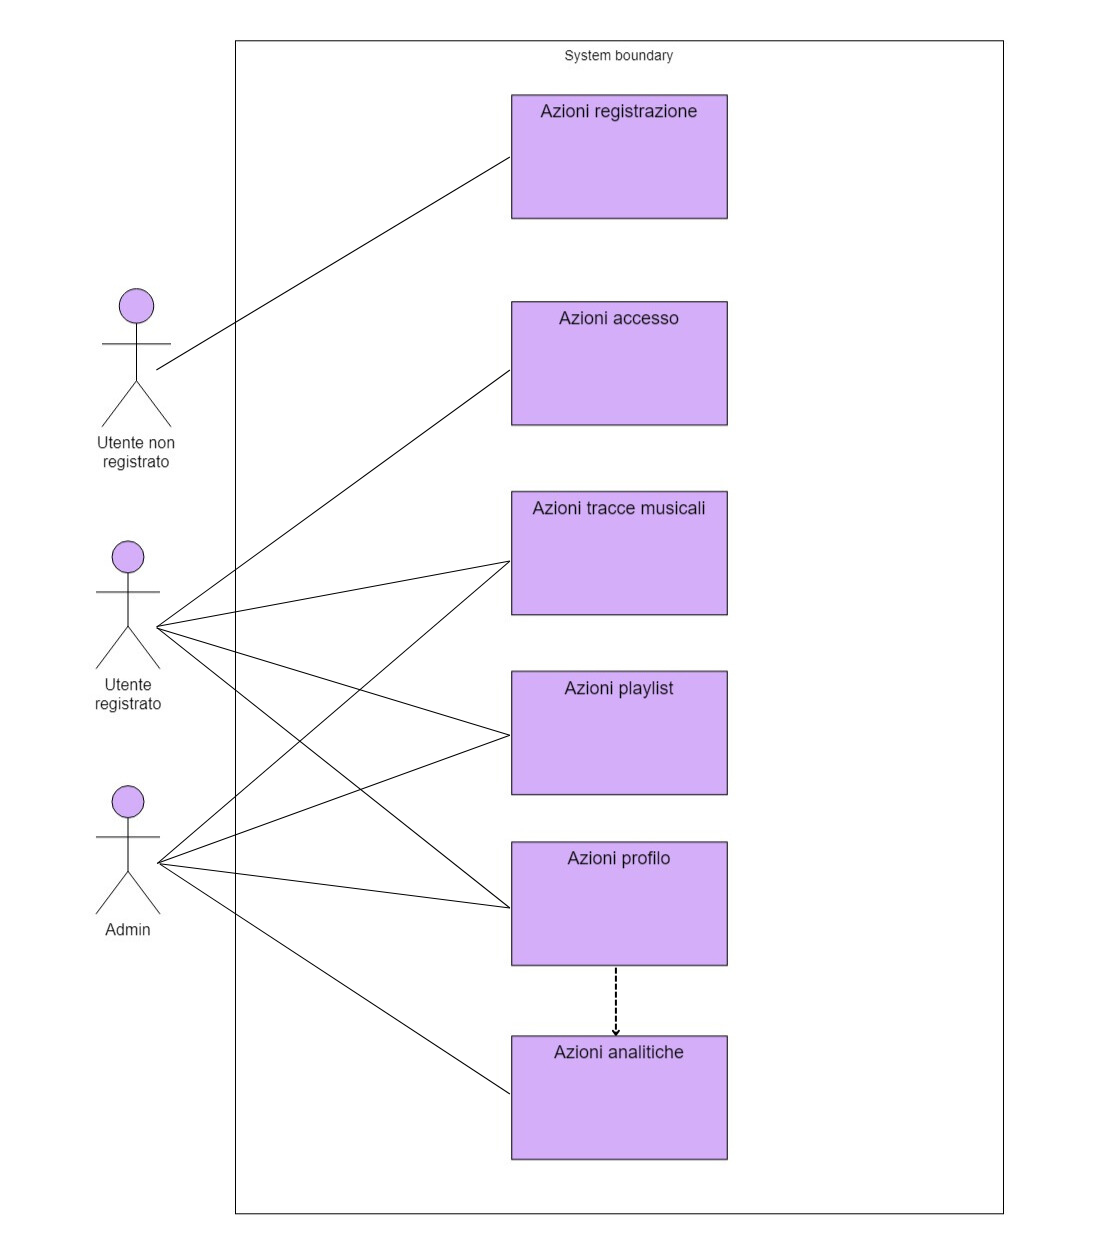
\includegraphics[width=0.8\textwidth]{usecasegenerale.png}
					\caption{Use Case Diagram generale}
				\end{figure}
				
			\subsubsection{Use Case azioni playlist}
			Nella seguente figura è descritto l'insieme delle azioni riguardanti le playlist.\\
			Si identificano le seguenti:
			\begin{itemize}
				\item Creare una nuova playlist
				\item Aggiungere un brano alla playlist
				\item Rimuovere un brano dalla playlist
				\item Rinominare una playlist
				\item Cambiare genere ad una playlist
				\item Aggiungere e/o rimuovere una playlist dalle preferite
				\item Eliminare una playlist
			\end{itemize}
			
			\begin{figure}[H]
				\centering
				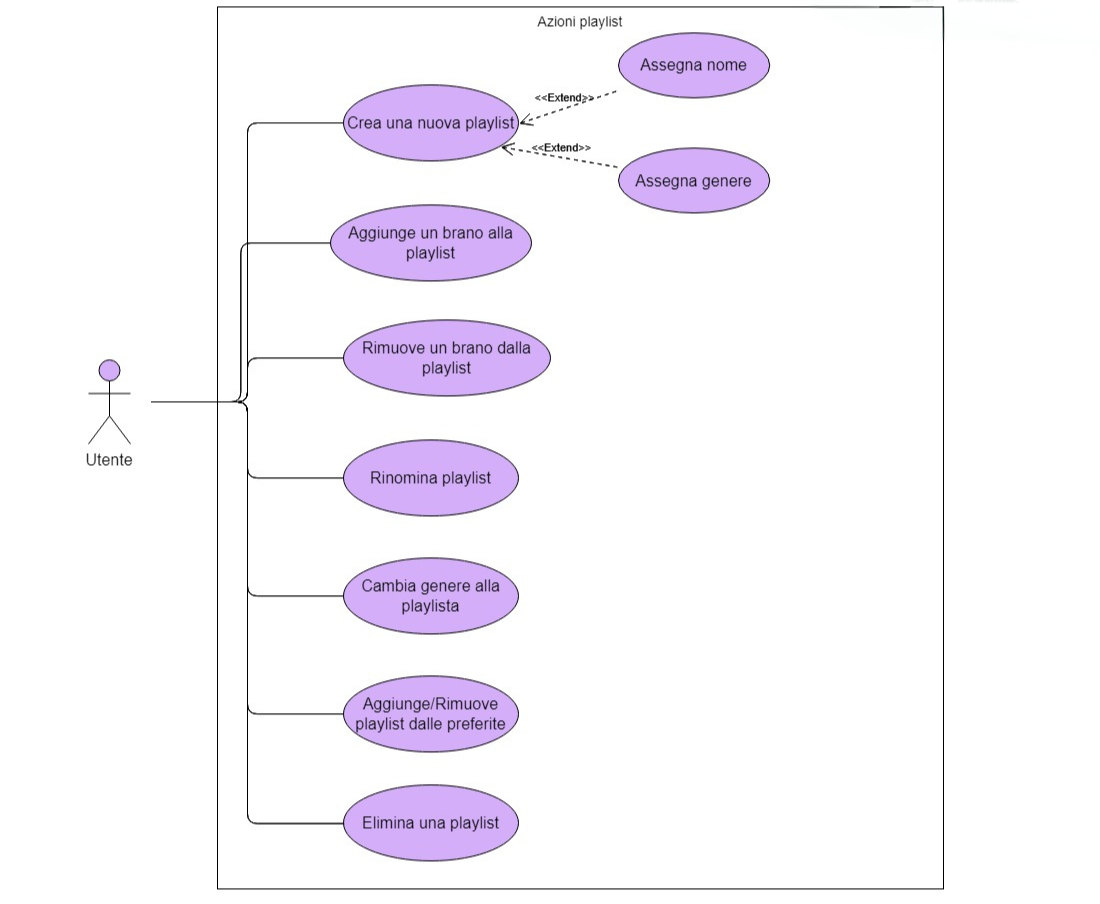
\includegraphics[width=0.9\textwidth]{Funzioniplaylist.png}
				\caption{Use Case Diagram azioni playlist}
			\end{figure}
			\subsubsection{Use Case aggiunta playlist ai preferiti}
			Nella seguente figura viene illustrato nel dettaglio il processo di aggiunta/rimozione di una playlist ai preferiti. L'utente, mediante l'utilizzo di un apposito toggle, può scegliere di includere o escludere tale playlist dall'elenco dei preferiti.
			
			\begin{figure}[H]
				\centering
				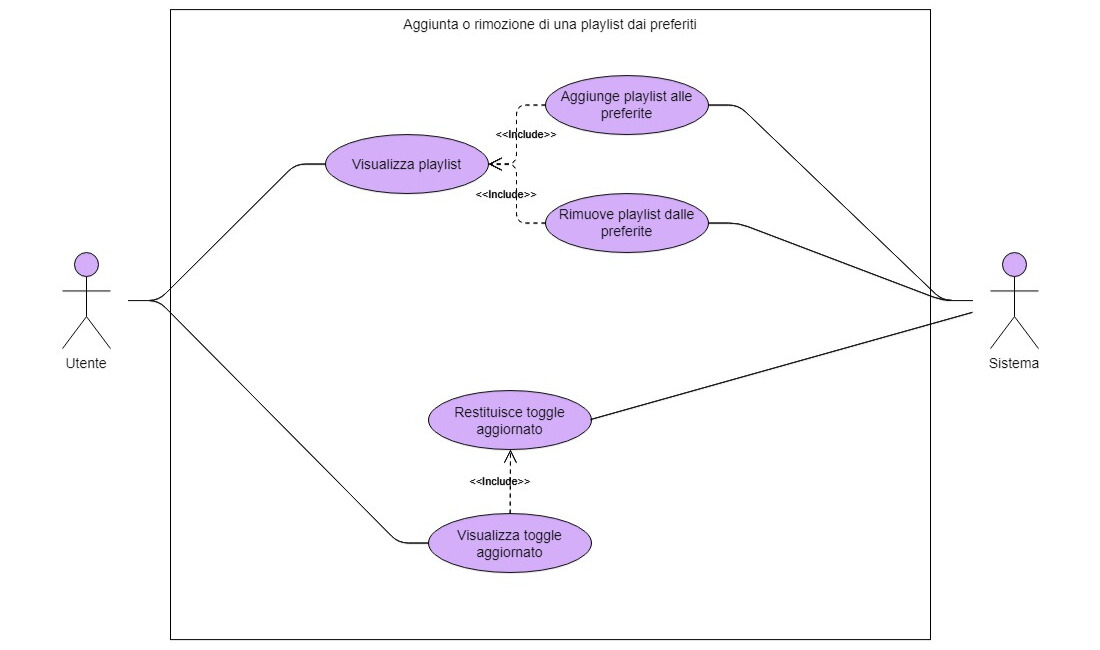
\includegraphics[width=0.9\textwidth]{aggiuntarimozione.png}
				\caption{Use Case Diagram aggiunta/rimozione playlist dai preferiti}
			\end{figure}
			\newpage
			\subsubsection{Use Case aggiunta brano dalla playlist}
			Nella seguente figura si è scelto di mostrare nel dettaglio l'aggiunta di una traccia musicale da una playlist.
			
			\begin{figure}[H]
				\centering
				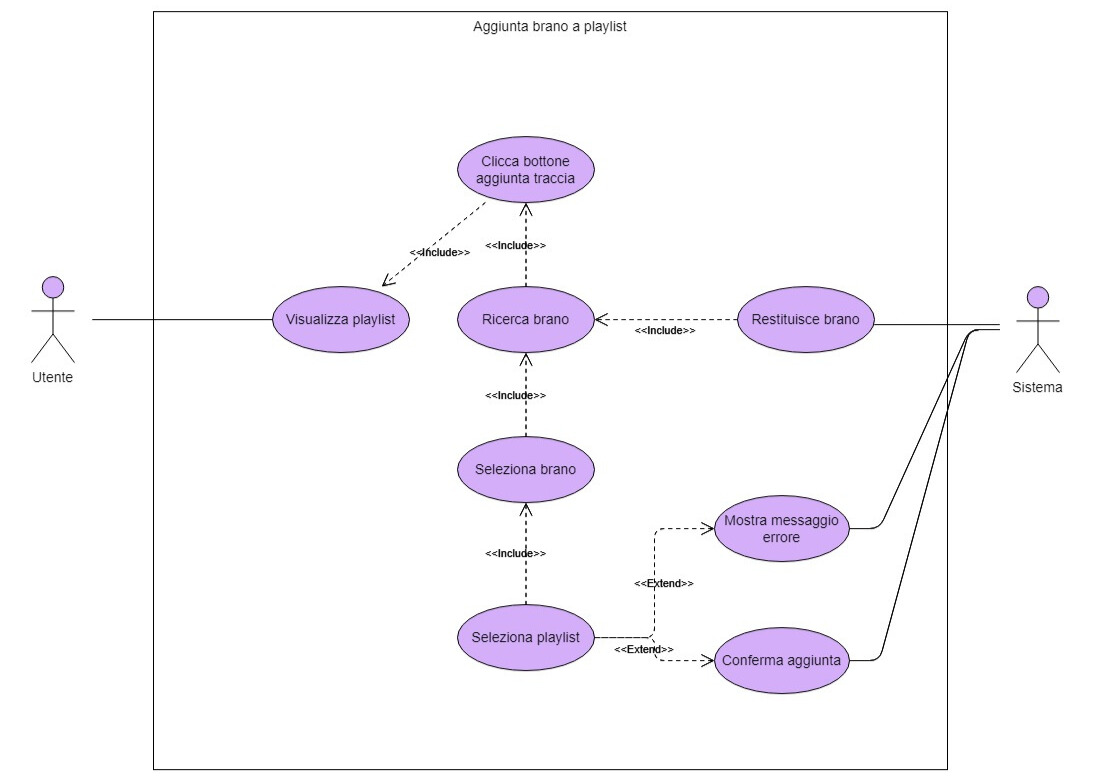
\includegraphics[width=0.9\textwidth]{aggiuntatraccia.png}
				\caption{Use Case Diagram aggiunta traccia musicale ad una playlist}
			\end{figure}
			
			\subsubsection{Use Case azioni analitiche}
			Il seguente use case rappresenta l'insieme di azioni che solamente l'utente admin può compiere.\\
			Le azioni in questione riguardano le analitiche:
			\begin{itemize}
				\item Se l'admin ricerca un utente, egli visualizzerà \textit{il numero di ascolti compiuti e la fascia oraria in cui ha utilizzato di più la piattaforma.}
				\item Se l'admin ricerca una traccia musicale, egli visualizzerà \textit{la tipologia della canzone, l'artista e il numero di ascolti totali del brano.}
				
				\begin{figure}[H]
					\centering
					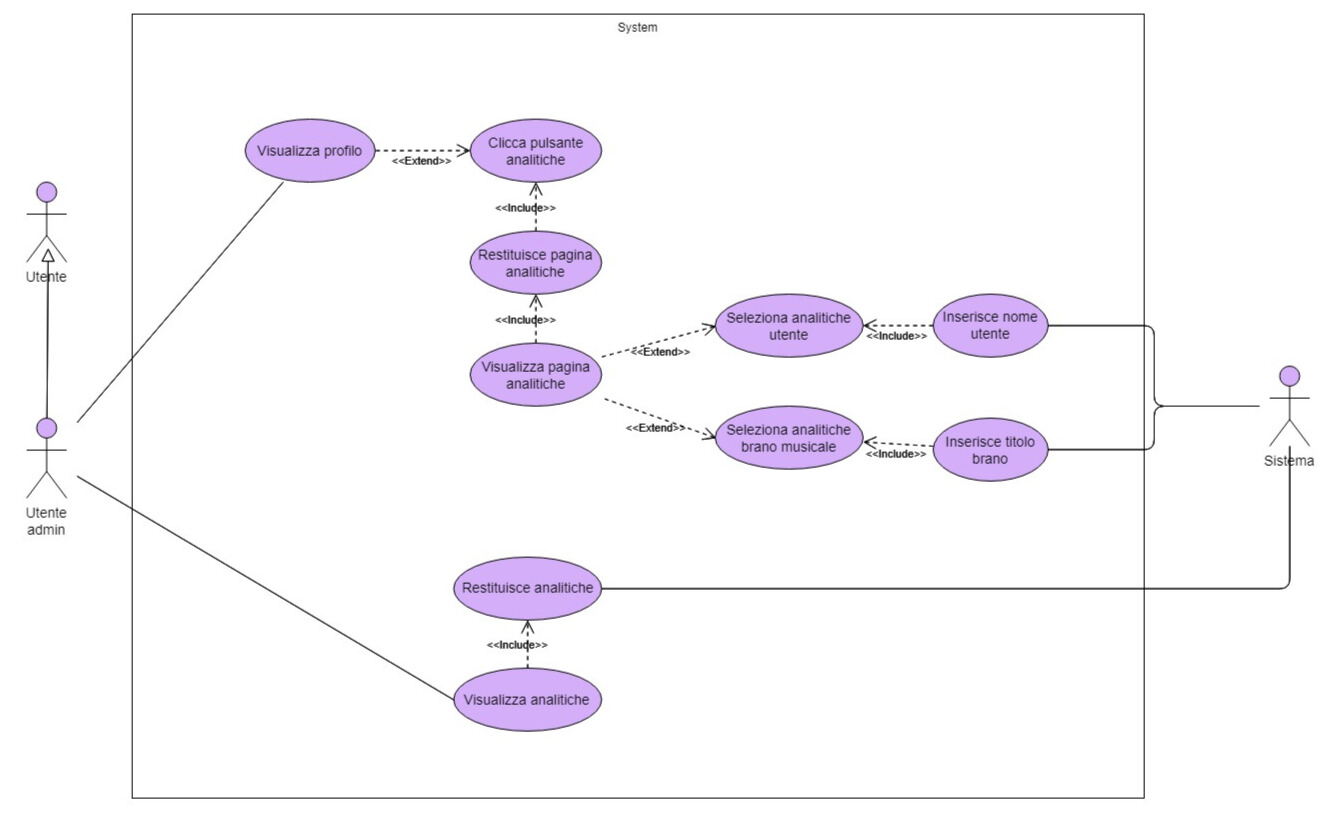
\includegraphics[width=0.9\textwidth]{analitiche.png}
					\caption{Use Case Diagram azioni analitiche}
				\end{figure}
			\end{itemize}
			\newpage
		\subsection{Tabelle di Cockburn}
		Le tabelle di Cockburn, che devono il loro nome all'informatico Alistair Cockburn, sono un formalismo di rappresentazione di casi d'uso; la politica adotta la rappresentazione di un \textit{main} scenario nella quale uno o più attori interagiscono tra loro attraverso l'invocazione di \textit{trigger} e descrivendo gli eventi (sottoforma tabulare).\\
		Abbiamo deciso di rappresentare i seguenti Use Case:
		\begin{itemize}
			\item Aggiunta canzone ad una playlist 
			\item Azioni analitiche (ricerca e visualizzazione)
		\end{itemize}
		\newpage
		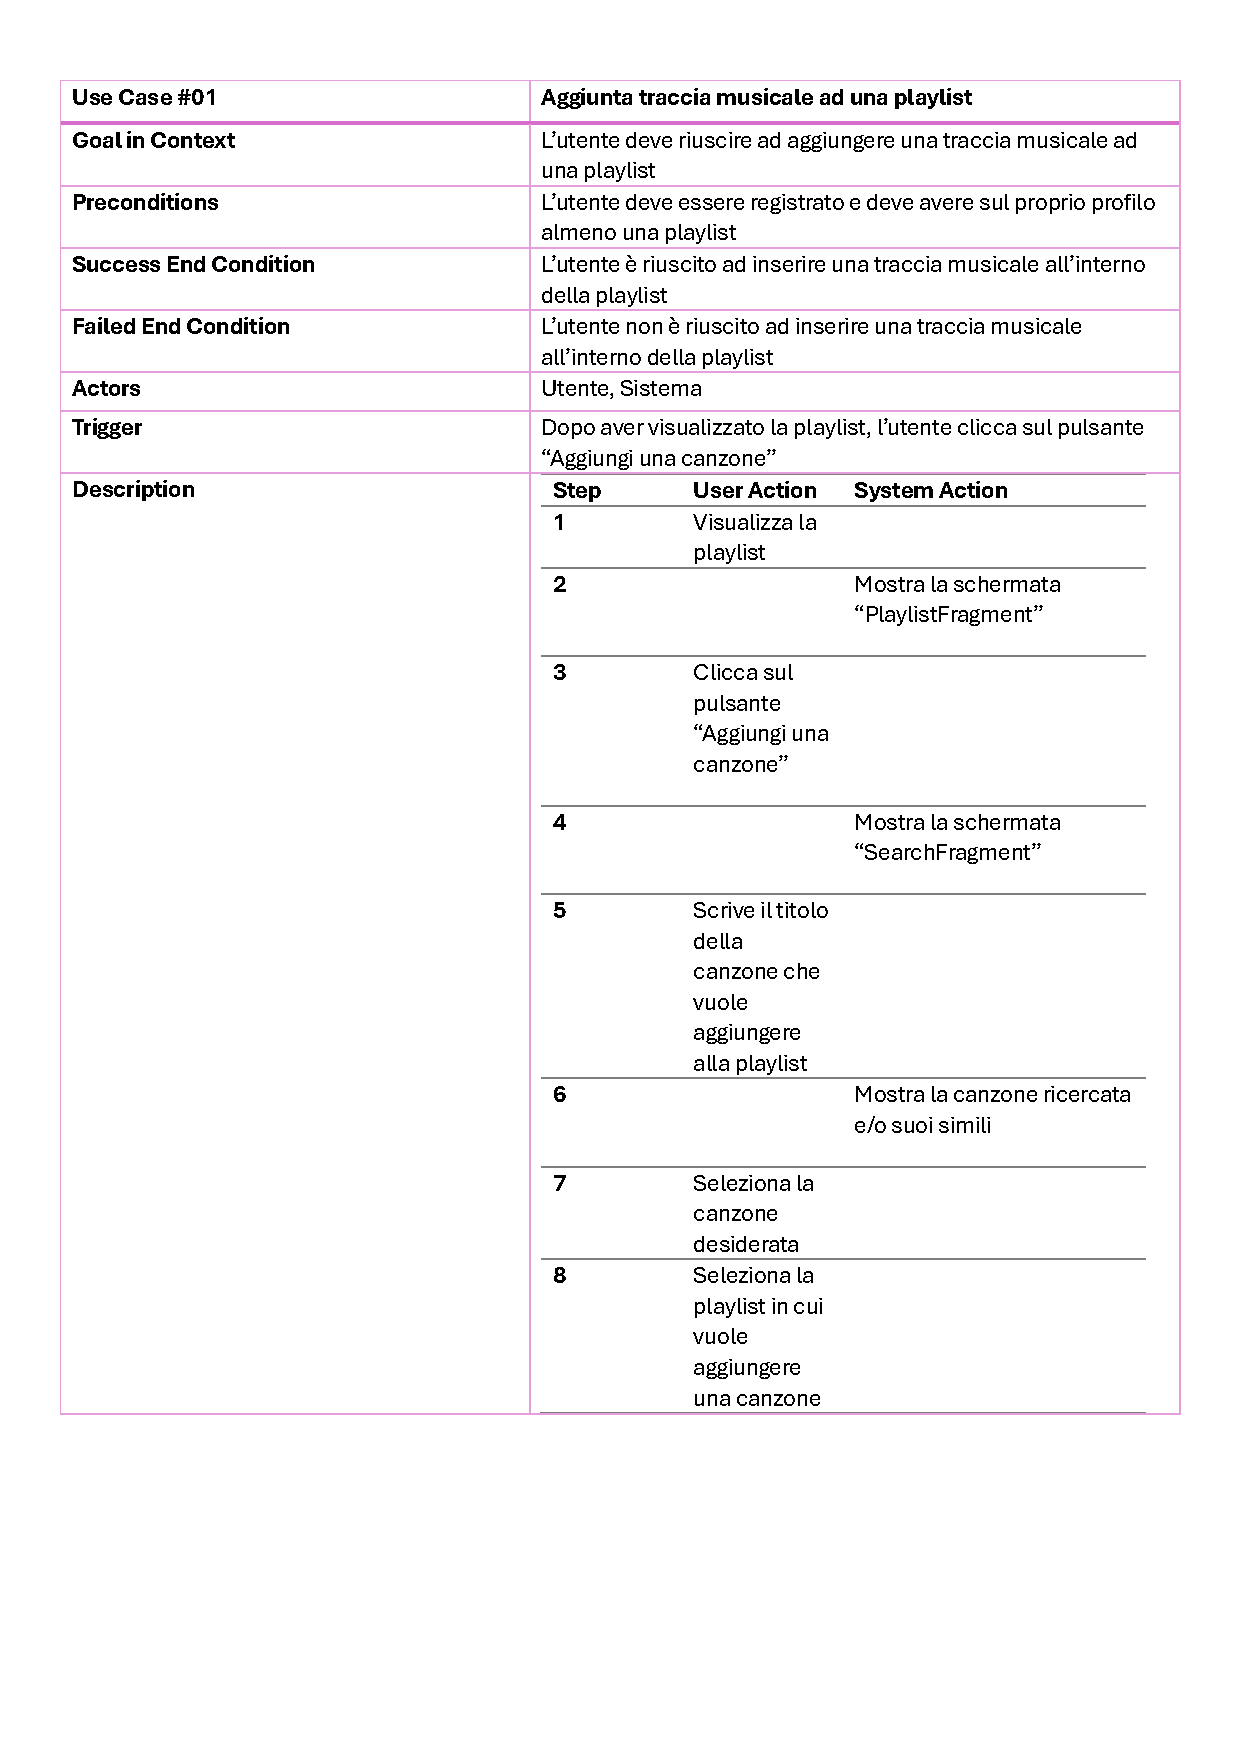
\includepdf[pages={1,2}]{usecase.pdf}
		\newpage
		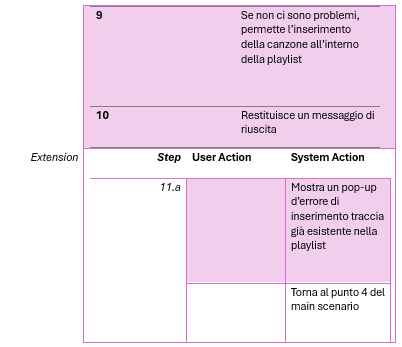
\includepdf[pages={1,2,3}]{Cockburn2}
		\newpage
		
		\subsection{UX Design}
		Il team ha approfondito diversi studi in materia di design della \textit{user experience} e implementato quelle che sono state ritenute le scelte migliori intermini di colori, affordances e estetica per assicurare all’utente la migliore esperienza possibile sull’applicativo.\\
		In termini di realizzazione pratica della GUI, la scelta è ricaduta:
		\begin{itemize}
			\item Coerenza visiva con altre applicazioni simili per facilitarne l'uso dell'interfaccia.
			\item Impatto estetico degli elementi
			\item Adattabilità delle sue componenti con il dispositivo usato
		\end{itemize}
		Per garantire una buona esperienza utente, si concorda sull'importanza di applicare i principi della \textbf{Gestalt}, una corrente psicologia tedesca dei primi del Novecento che costruisce l'esperienza rispetto a diversi fenomeni. 
		\\Secondo la \textit{Gestalt} gli elementi simili che costituiscono un'immagine o una composizione, vengono raggruppati tra loro e poi percepiti come un unico elemento.
		\begin{figure}[H]
			\centering
			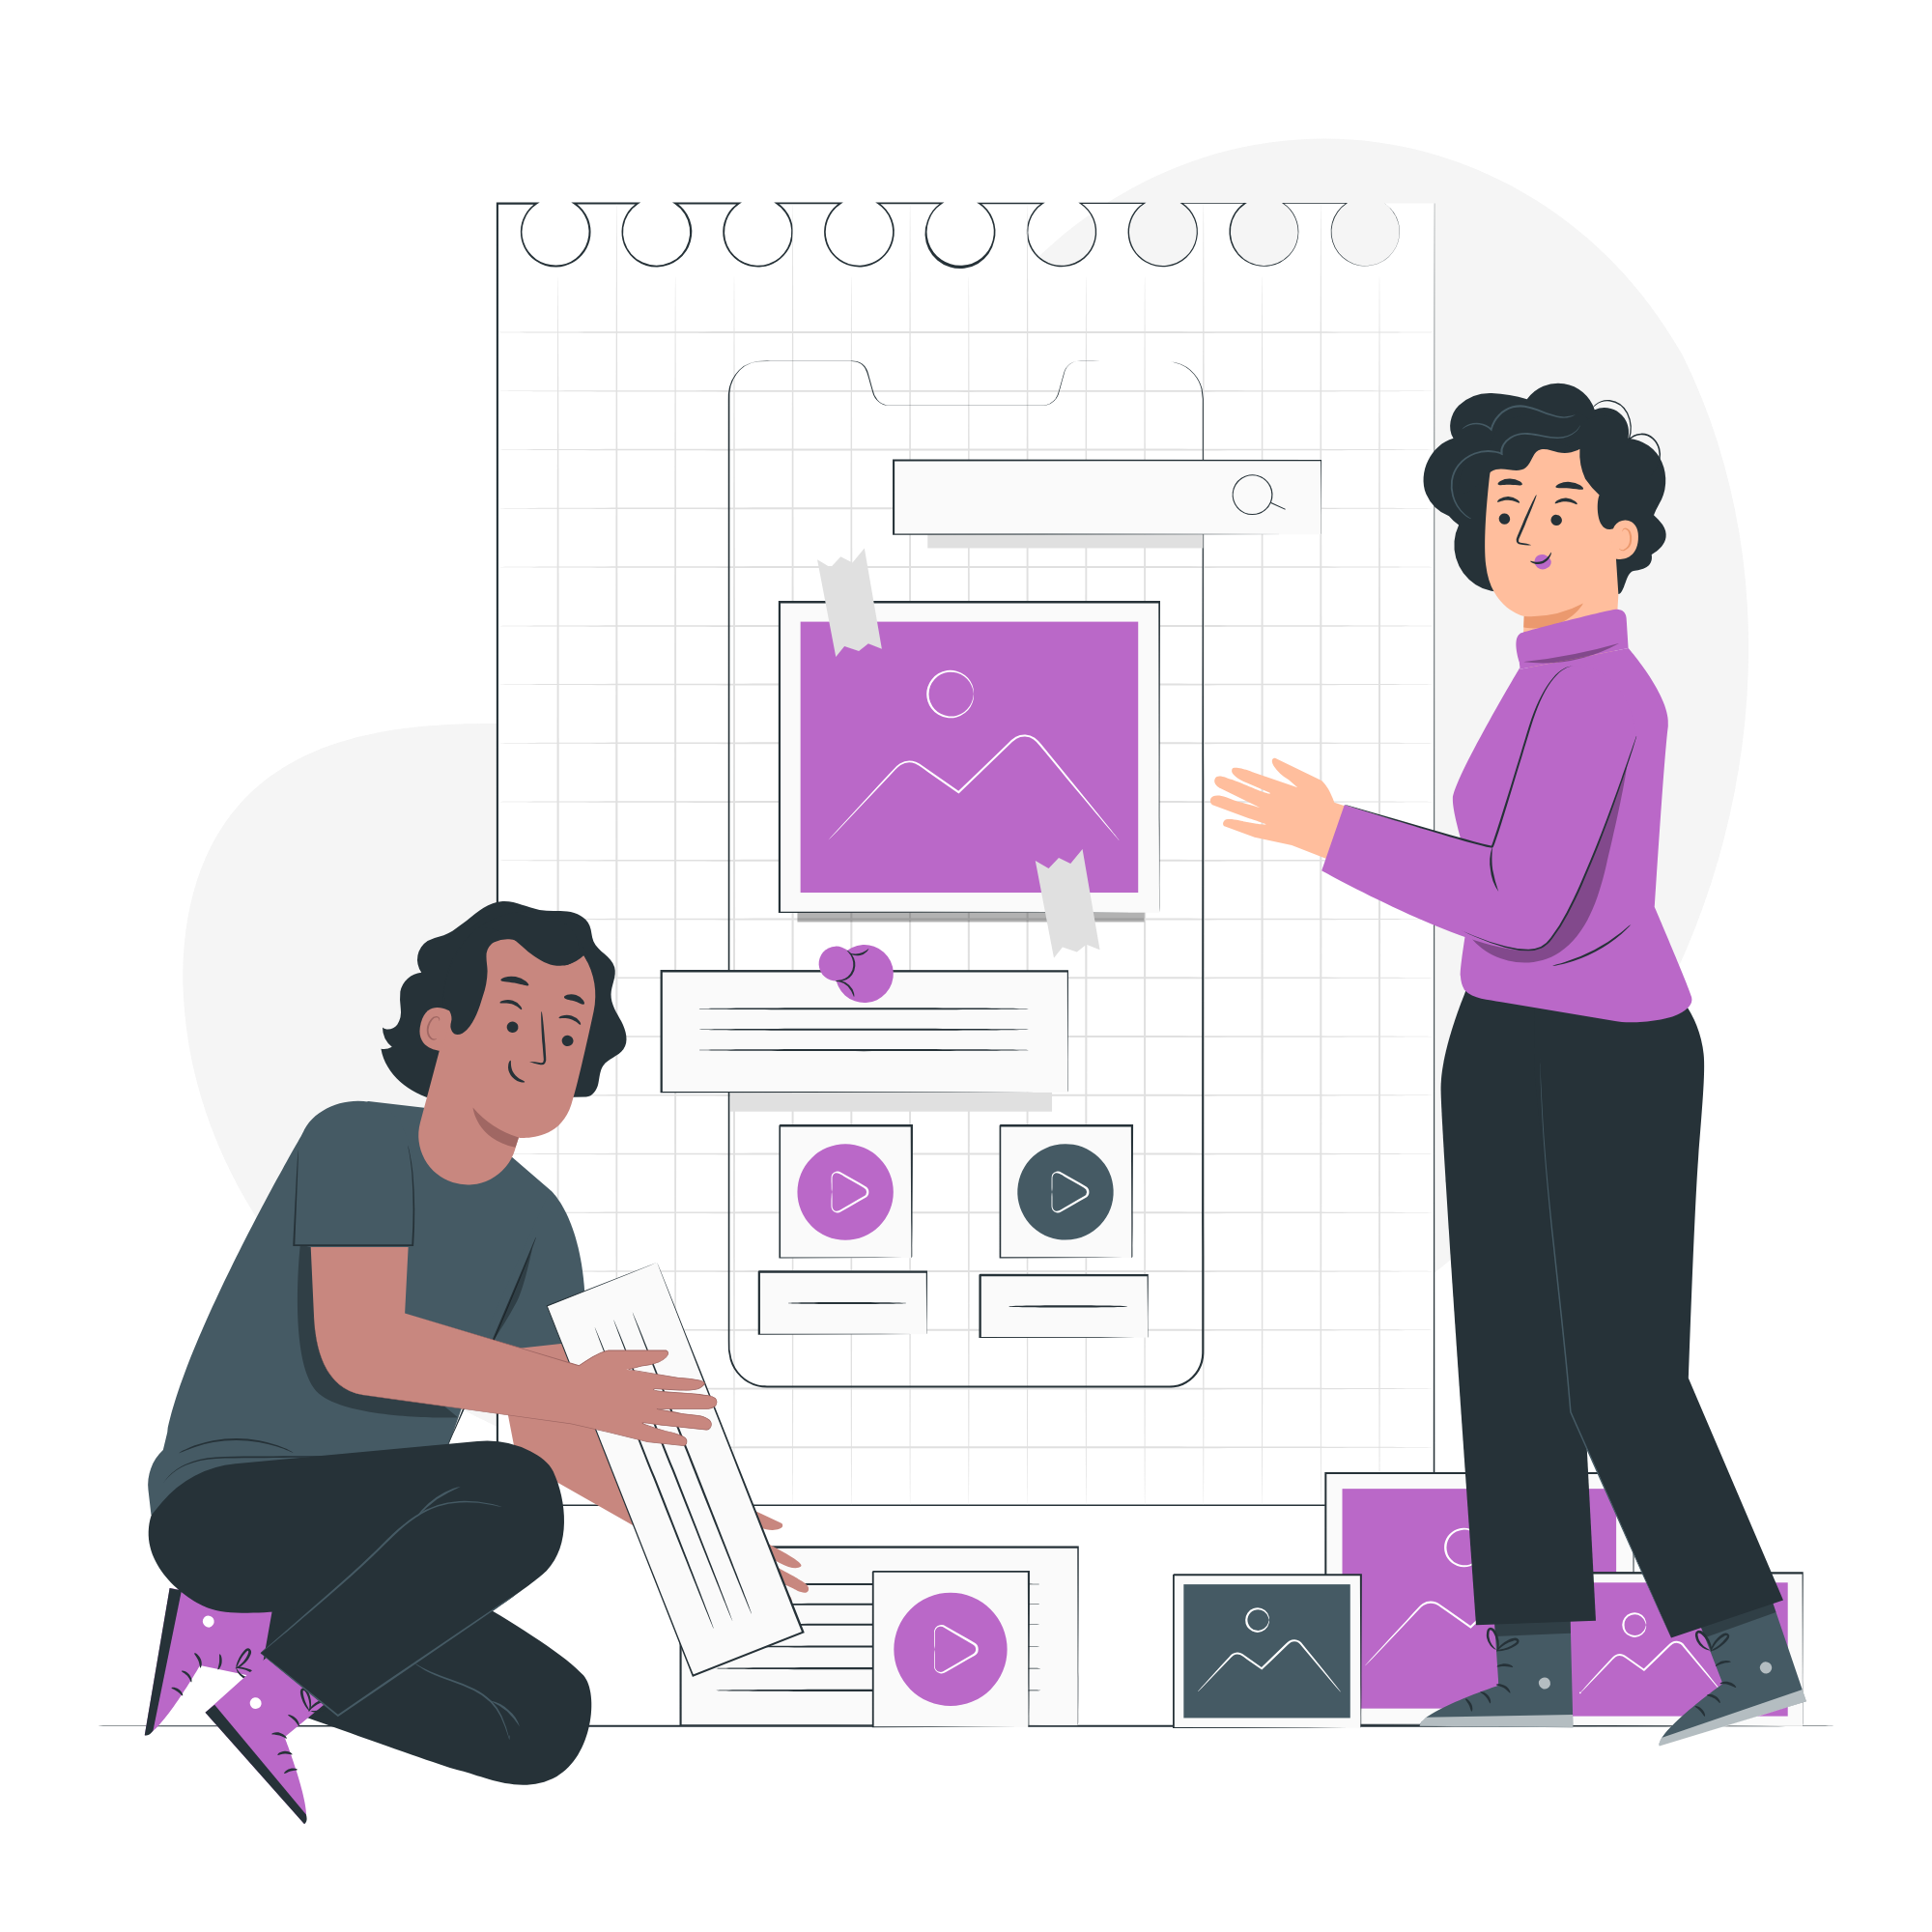
\includegraphics[width=0.6\textwidth]{uxdesign.png}
		\end{figure}
		\textbf{Il colore e le forme} hanno, dunque, un ruolo importantissimo nella creazione di un'interfaccia utente in quanto non solo migliora l'estetica ma è un veicolo di informazioni.
		La palette colori che abbiamo deciso di utilizzare per il nostro applicativo è la seguente:
		\begin{figure}[H]
			\centering
			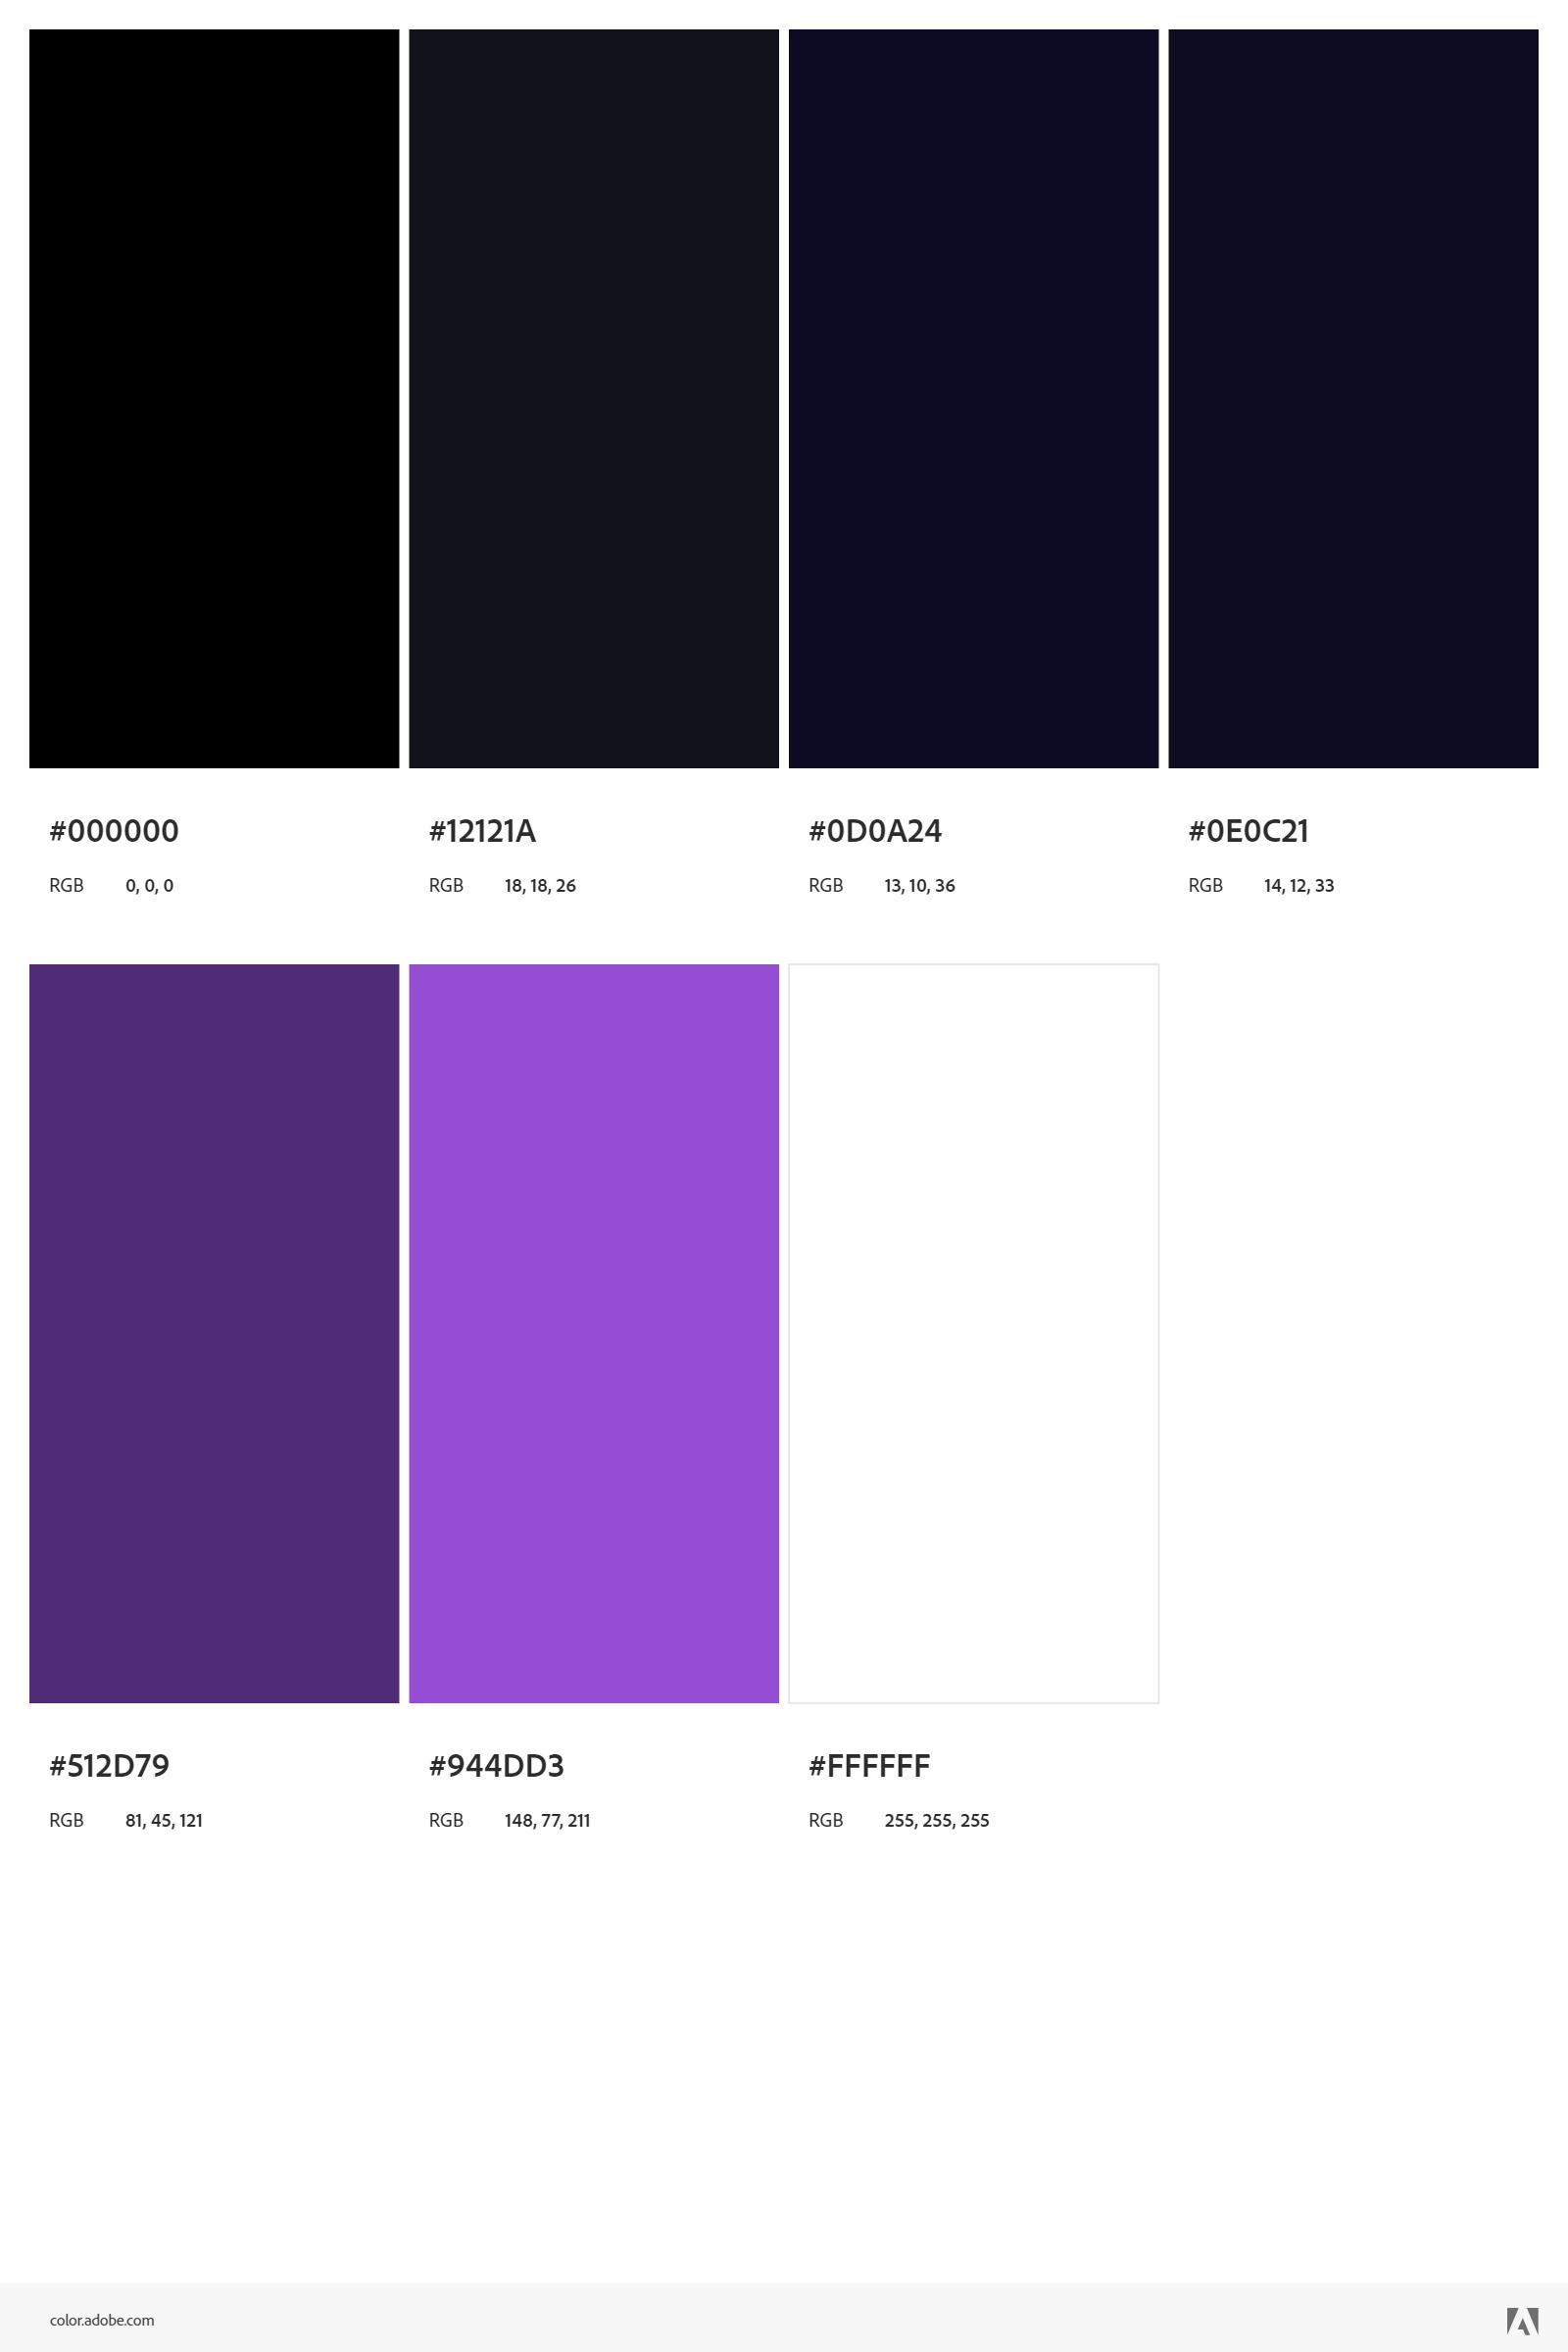
\includegraphics[width=0.6\textwidth]{palette}
		\end{figure}
		La scelta di tale palette colori nasce dal nome stesso dell'applicativo:
		\begin{itemize}
			\item \textbf{Sound:} traduzione in inglese della parola "suono"
			\item \textbf{Lab:} diminutivo della parola inglese "Laboratory"
		\end{itemize}
		La scelta delle sfumature del color viola affiancate ai classici bianco e nero, rappresentano una forte connessione al mondo della musica ma anche al tema del laboratorio su cui verte l'applicativo.
		\begin{itemize}
			\item \textbf{Viola:} spesso associato alla creatività, all'innovazione e alla magia. Questi attributi sono fondamentali laddove si vogliano esplorare nuove idee, facendo della creatività il fulcro della composizione e dell'espressione artistica.
			\item \textbf{Nero:} colore elegante e sofisticato, che dona un aspetto raffinato e professionale. Inoltre, il nero può aiutare a mantenere il focus sugli elementi principali dell'interfaccia senza distrazioni.
			\item \textbf{Bianco:} offre un ottimo contrasto con i colori più scuri della palette, migliorando la leggibilità del testo e la visibilità degli elementi interattivi.
		\end{itemize}
		La scelta di utilizzare \textbf{forme} più tondeggianti rispetto a quelle spigolose in termini di estetica ed usabilità può influenzare significativamente l'esperienza utente.
		\begin{itemize}
			\item Le forme tondeggianti sono spesso percepite come più morbide e accoglienti rispetto a quelle spigolose.\\ Questo può creare un'atmosfera più amichevole e invitante per l'utente, contribuendo a rendere l'app più piacevole e meno intimidatoria
			\item Le curve e le linee arrotondate sono caratteristiche comuni nel design moderno e contemporaneo. \\Questi elementi possono dare all'app un aspetto più aggiornato e all'avanguardia, in linea con le tendenze attuali del design
			\item Le forme tondeggianti possono creare un senso di continuità e flusso visivo. La transizione tra gli elementi è più fluida, contribuendo a un'interfaccia più armoniosa e integrata
			\item Le forme tondeggianti possono trasmettere una sensazione di sicurezza e protezione, in quanto mancano degli angoli appuntiti che potrebbero sembrare minacciosi. \\Questo può essere particolarmente importante per utenti con esigenze di accessibilità, rendendo l'app più inclusiva
		\end{itemize}
		Fin dal prototipo iniziale, i valori citati precedentemente sono stati sempre rispettati.
		Bisogna specificare, però, che in fase di sviluppo molte scelte stilistiche sono state modificate per garantire una funzionalità maggiore dell'applicativo. 
		\hspace{0.1\textwidth}
		\begin{center}
			\begin{figure}[htbp]
				\centering
				\begin{minipage}[t]{0.2\textwidth}
					\centering
					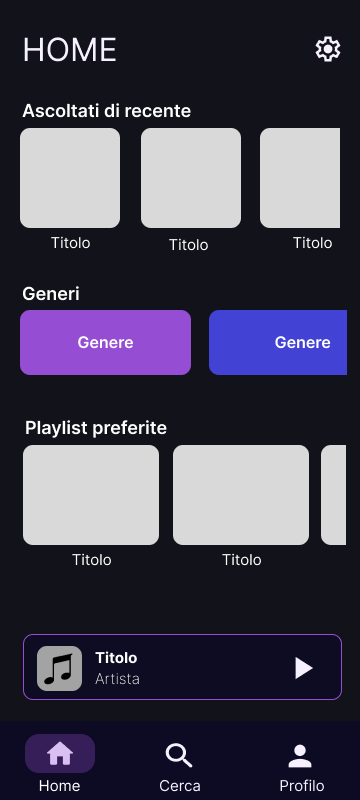
\includegraphics[width=\textwidth]{home_page}
					\caption{Prototipo iniziale della schermata di home}
					\label{fig:home_page}
				\end{minipage}%
				\hspace{0.1\textwidth}
				\begin{minipage}[t]{0.2\textwidth}
					\centering
					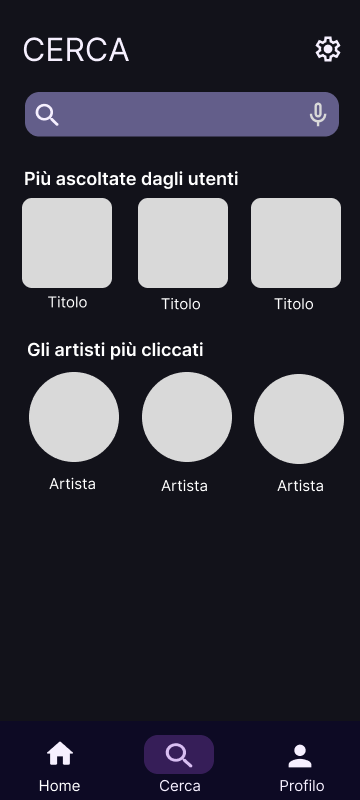
\includegraphics[width=\textwidth]{search_page}
					\caption{Prototipo iniziale della pagina di ricerca}
					\label{fig:search_page}
				\end{minipage}
			\end{figure}
		\end{center}
		\newpage
		
			\subsubsection{Mockup}
			Il mockup è una rappresentazione visiva del prodotto o dell’idea, utilizzata per valutarne l’aspetto e l’organizzazione. È un modello statico e illustra l’aspetto e il funzionamento previsto di un prodotto, per esempio.\\
			Esso comprende elementi, come per esempio l’aspetto grafico (i loghi, le immagini, i colori, le visualizzazioni della navigazione, ecc.), che saranno utilizzati nel design finale e nell’esperienza dell’utente.
			In sostanza, un mockup serve a mostrare agli stakeholder e agli utenti come potrebbe essere il progetto o il prodotto finito, offrendone un’idea visiva chiara e dettagliata del design e delle funzionalità.\\
			I mockup sono stati fatti utilizzando come tool-case \textbf{Figma}. Di seguito, una prima versione del \textit{mockup}\footnote{L'applicativo finale rispecchia in pieno i mockup iniziali. Tuttavia, bisogna specificare che in fase di sviluppo alcune scelte stilistiche sono state modificate per favorire la user experience}.
			\begin{figure}[htbp]
				\centering
				\begin{minipage}{0.18\textwidth}
					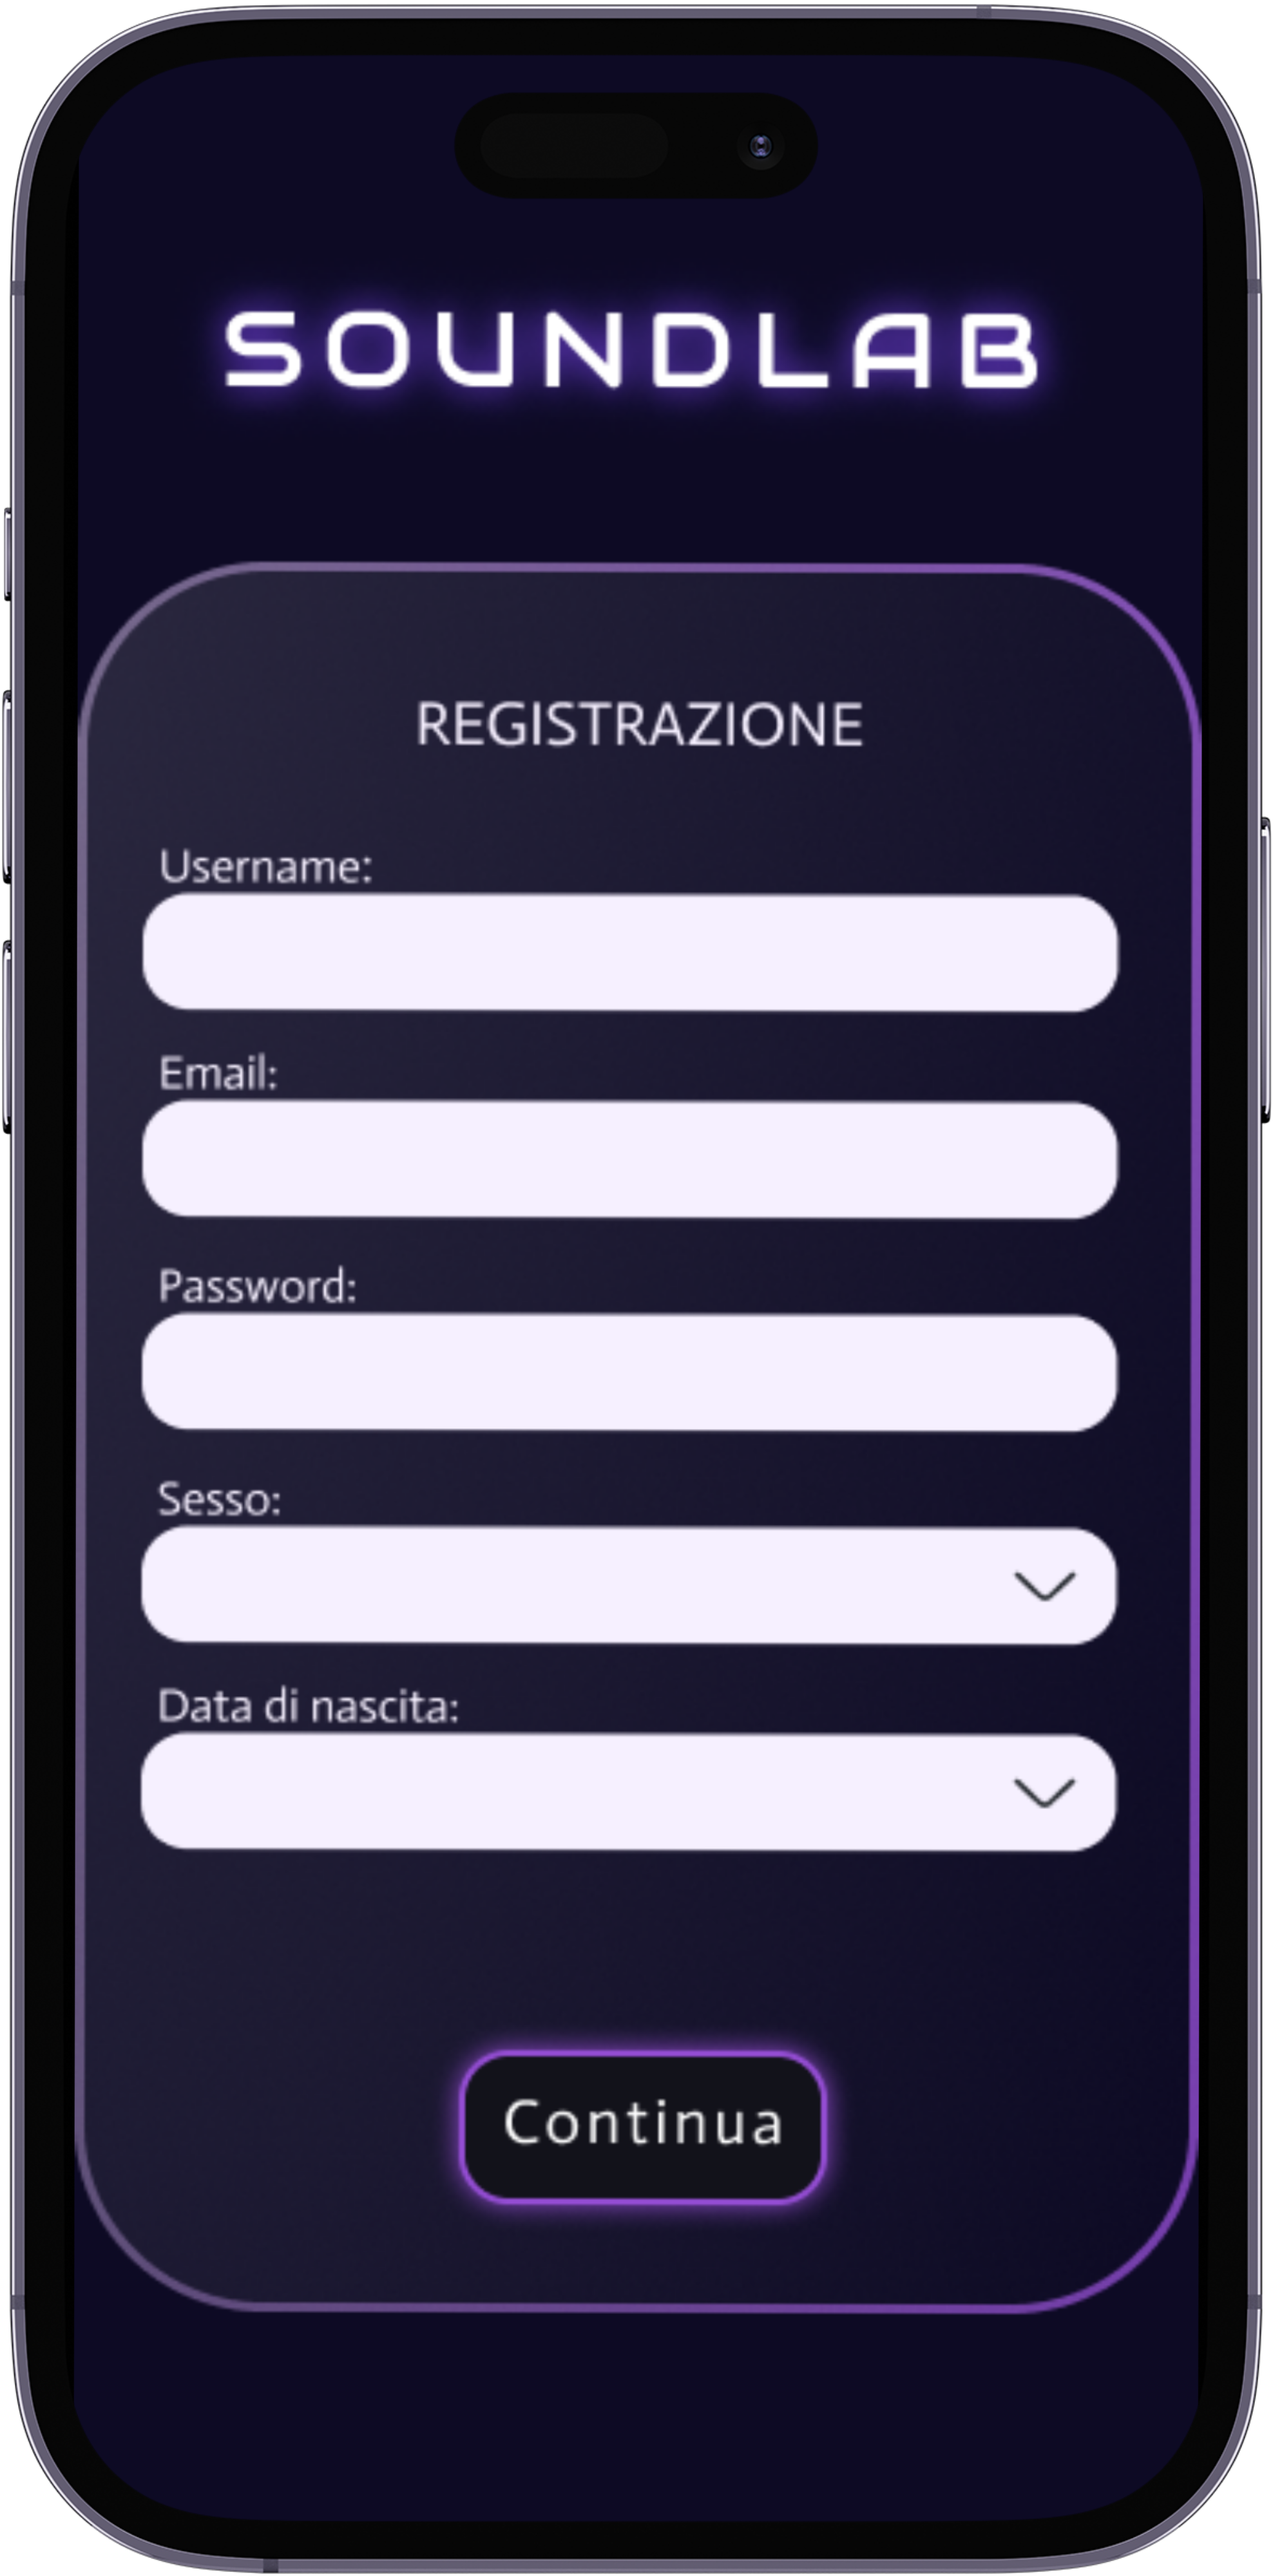
\includegraphics[width=\textwidth]{foto1}
				\end{minipage}
				\hfill
				\begin{minipage}{0.18\textwidth}
					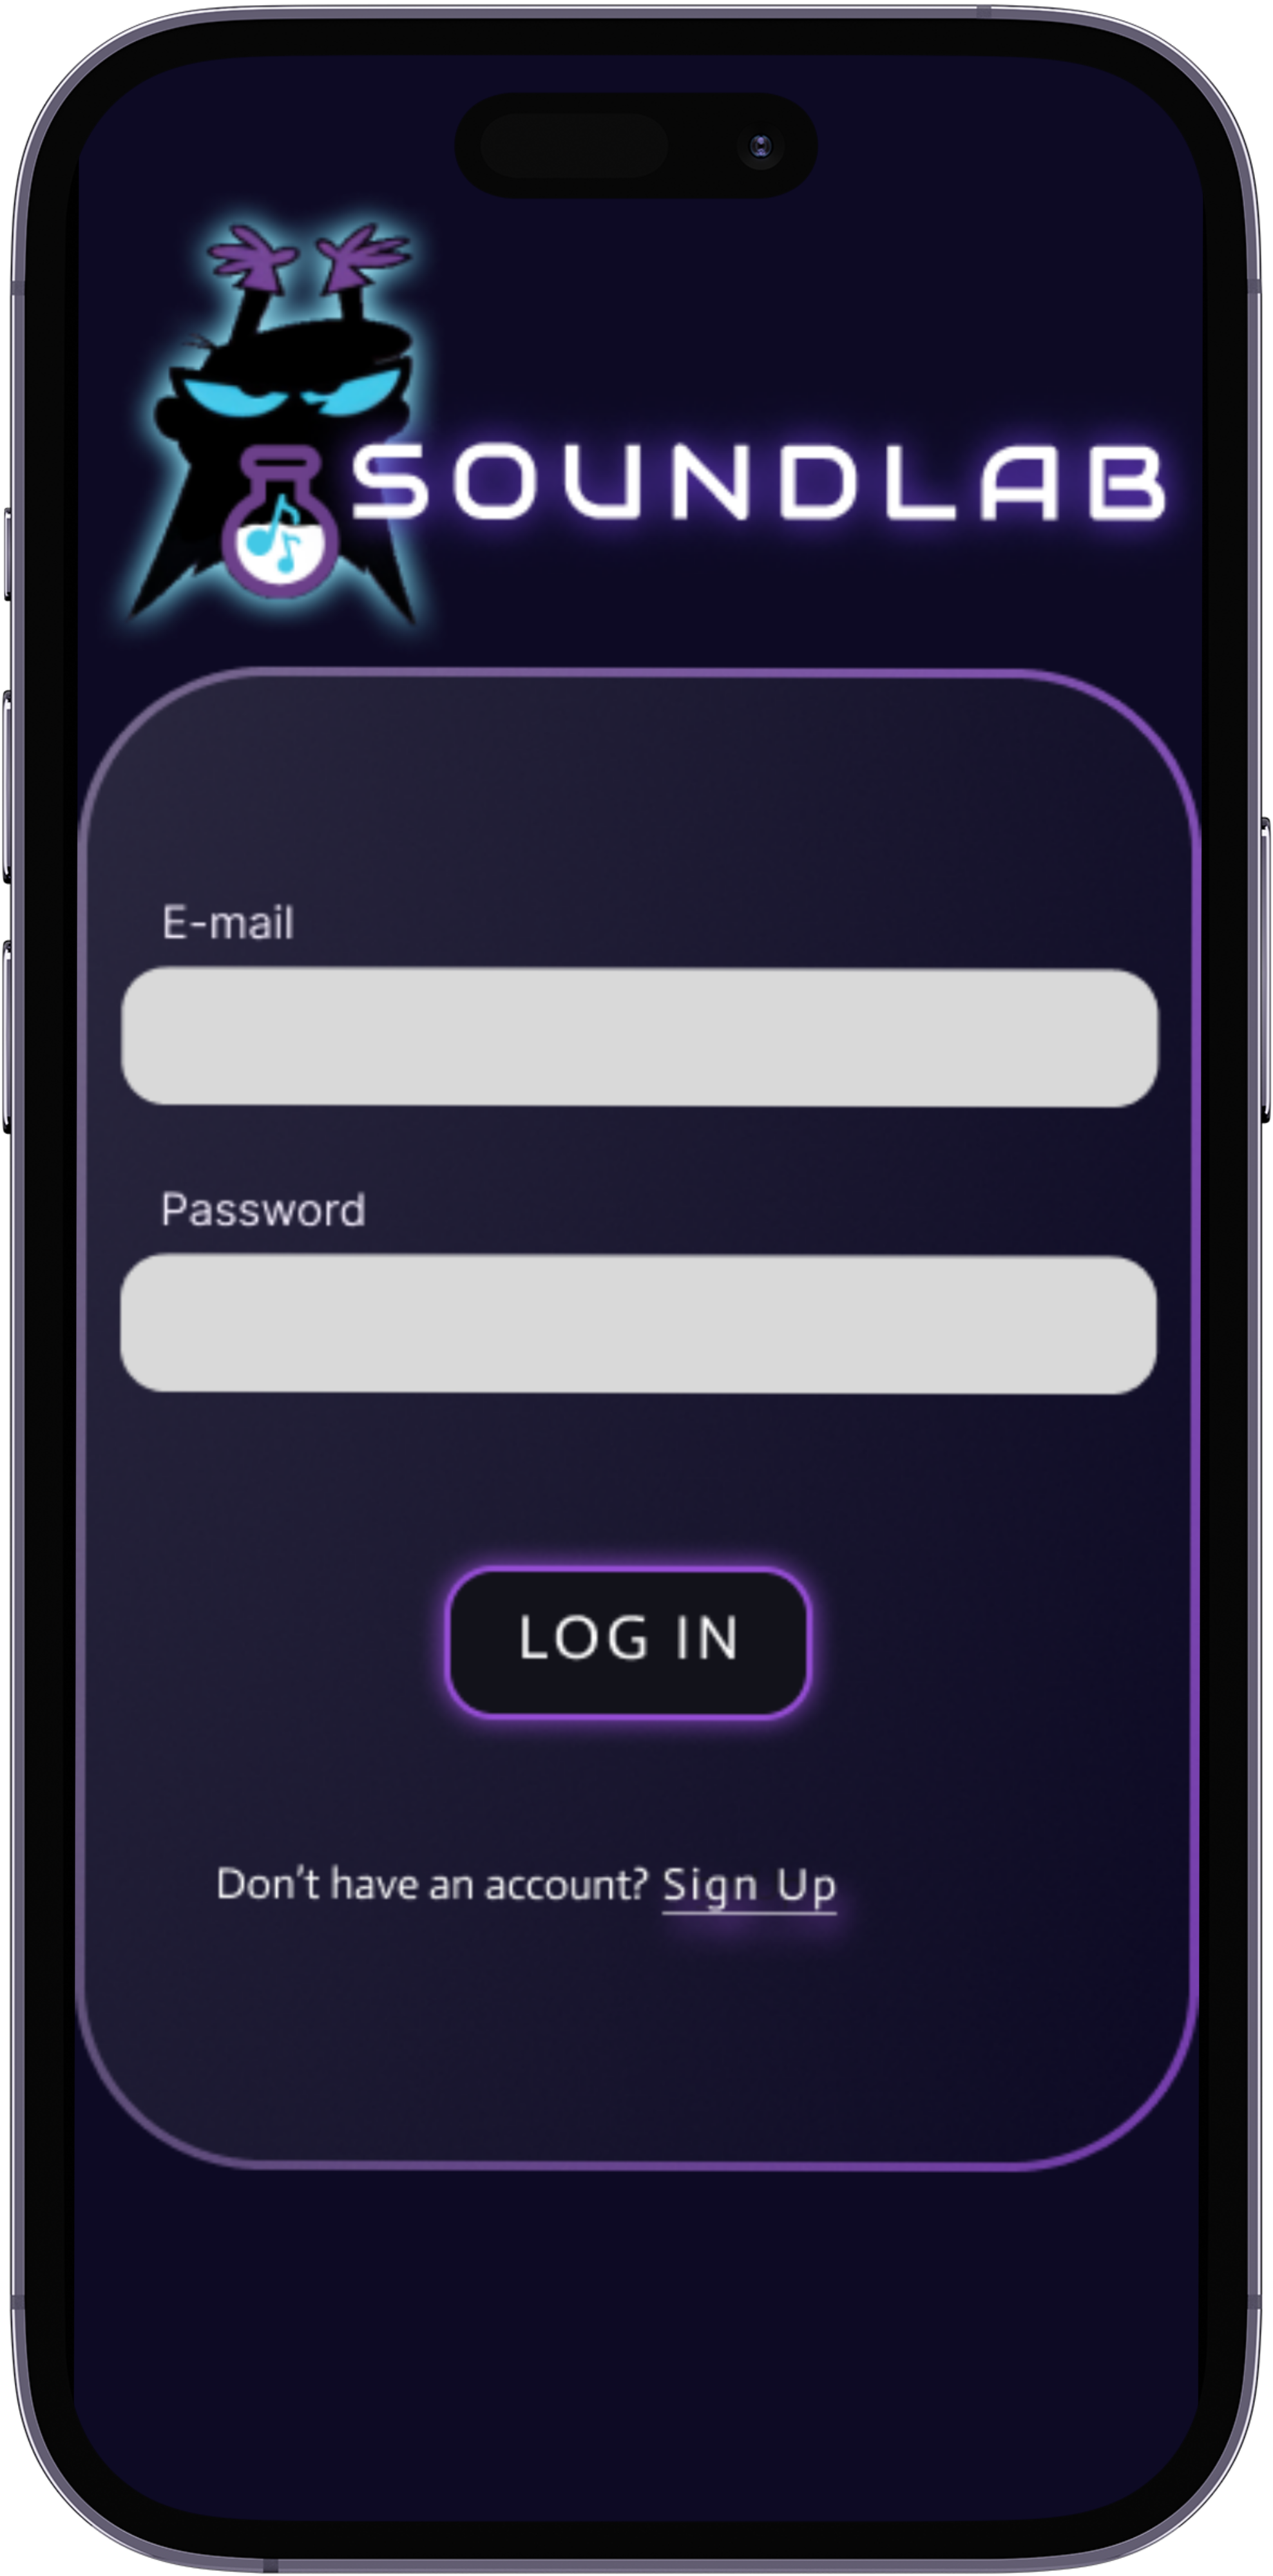
\includegraphics[width=\textwidth]{foto2}
				\end{minipage}
				\hfill
				\begin{minipage}{0.18\textwidth}
					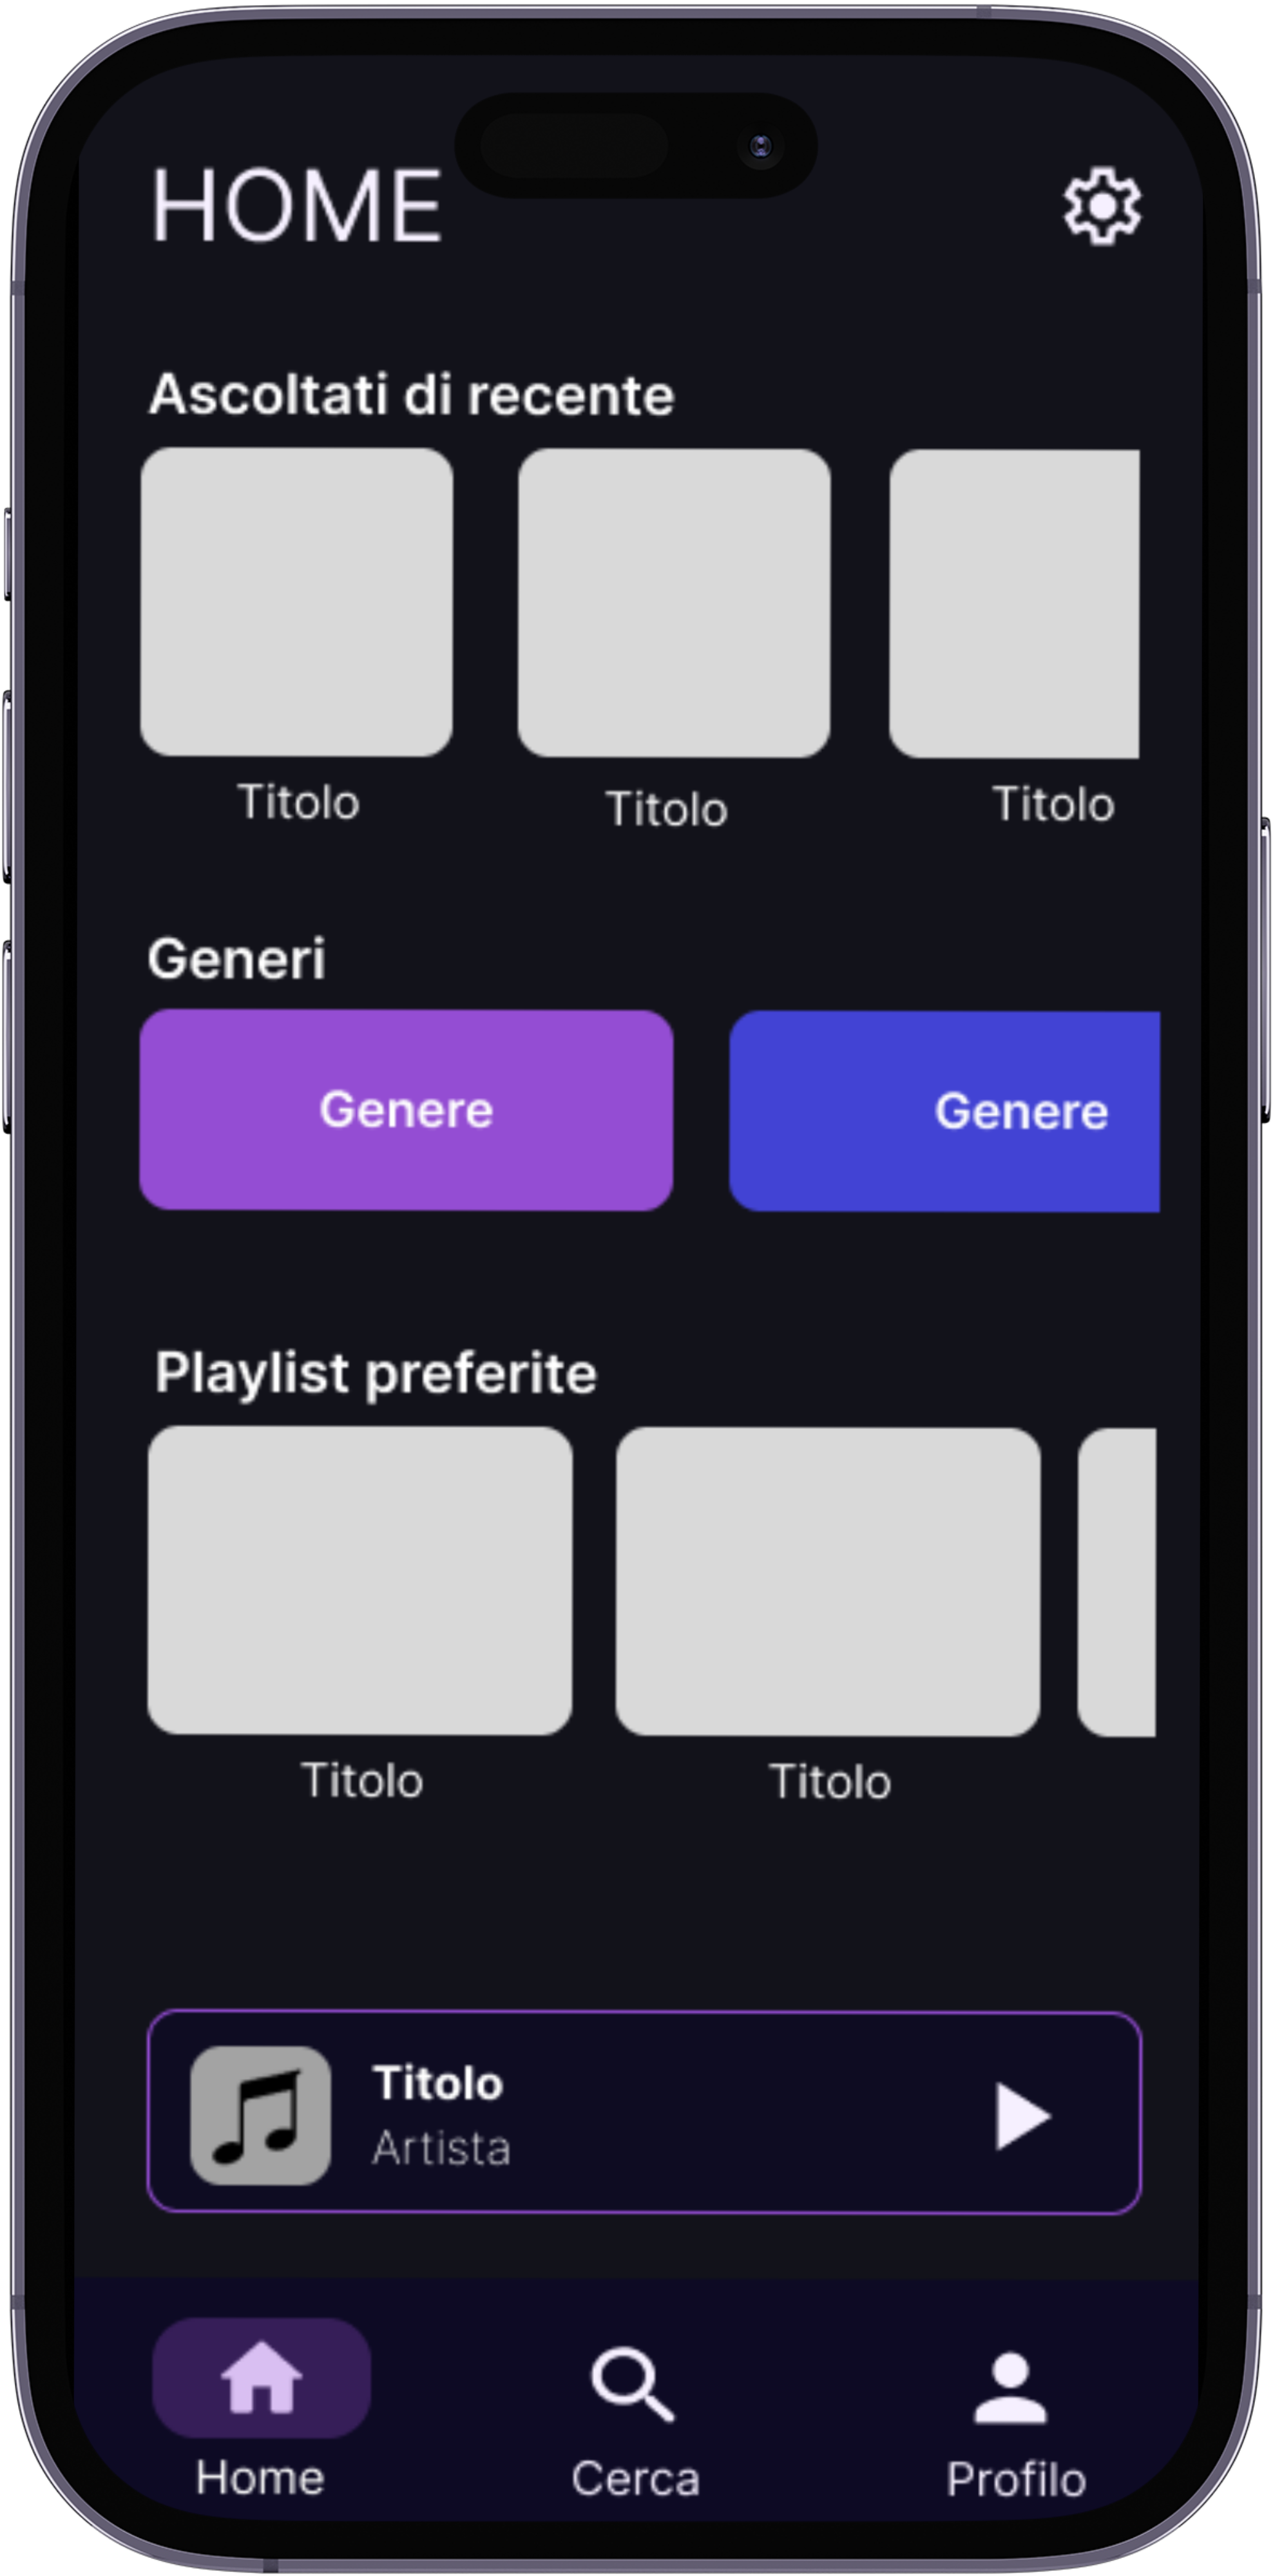
\includegraphics[width=\textwidth]{foto3}
				\end{minipage}
				\hfill
				\begin{minipage}{0.18\textwidth}
					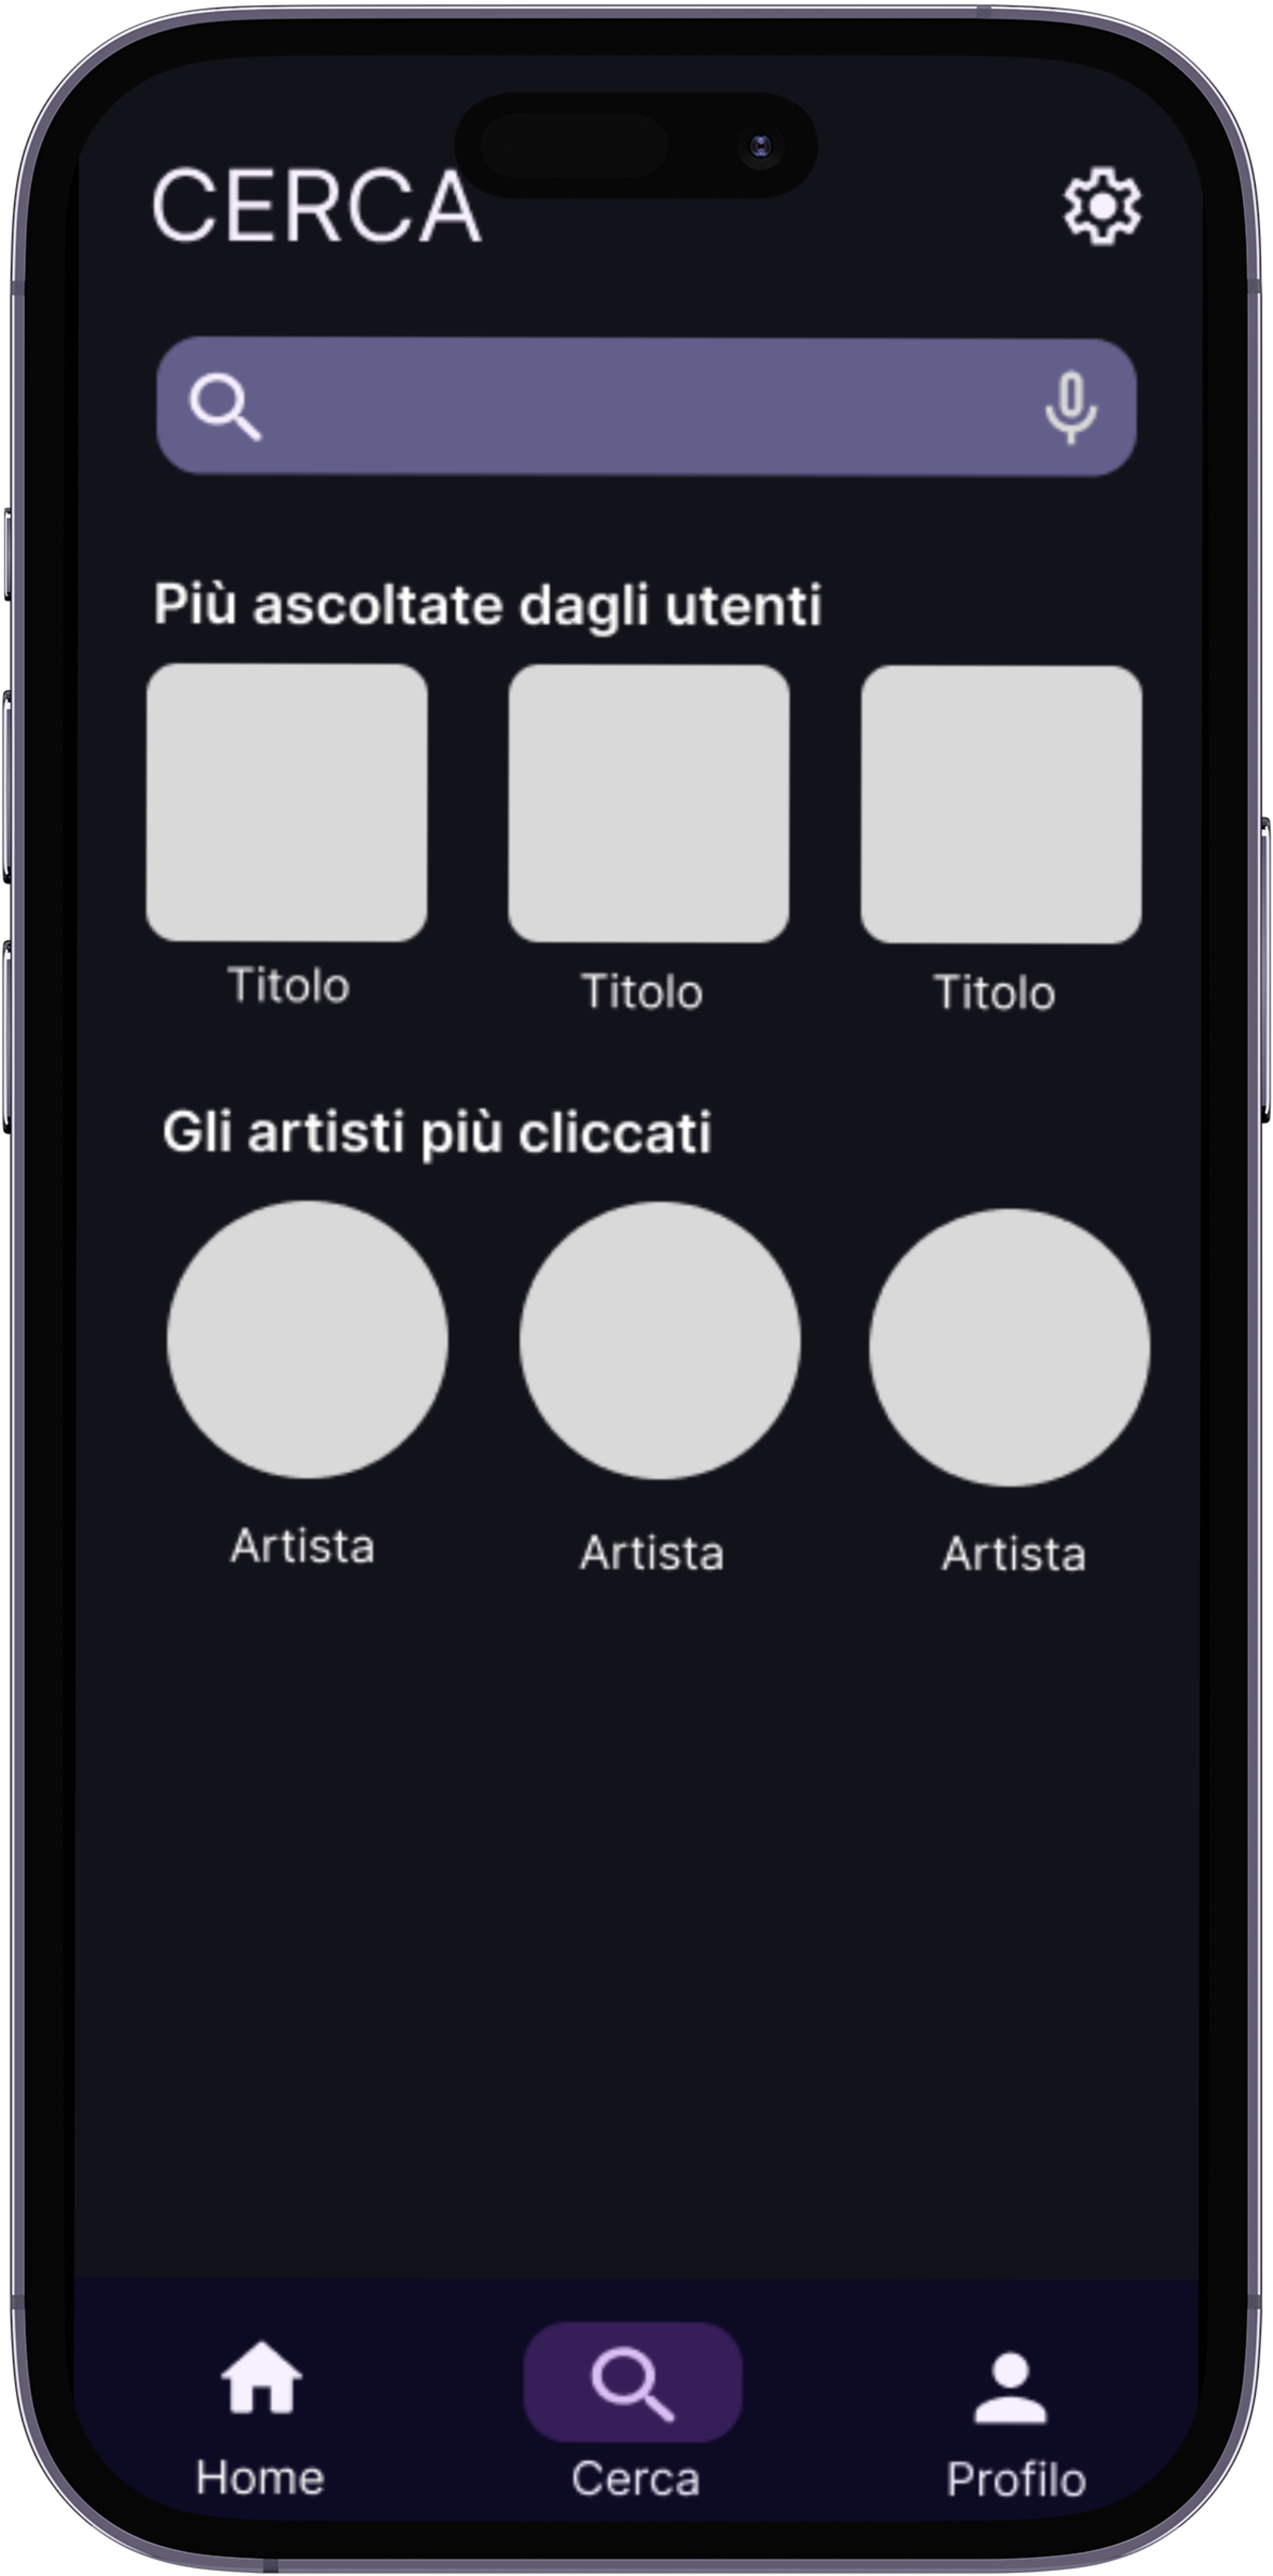
\includegraphics[width=\textwidth]{foto4}
				\end{minipage}
				\hfill
				\begin{minipage}{0.18\textwidth}
					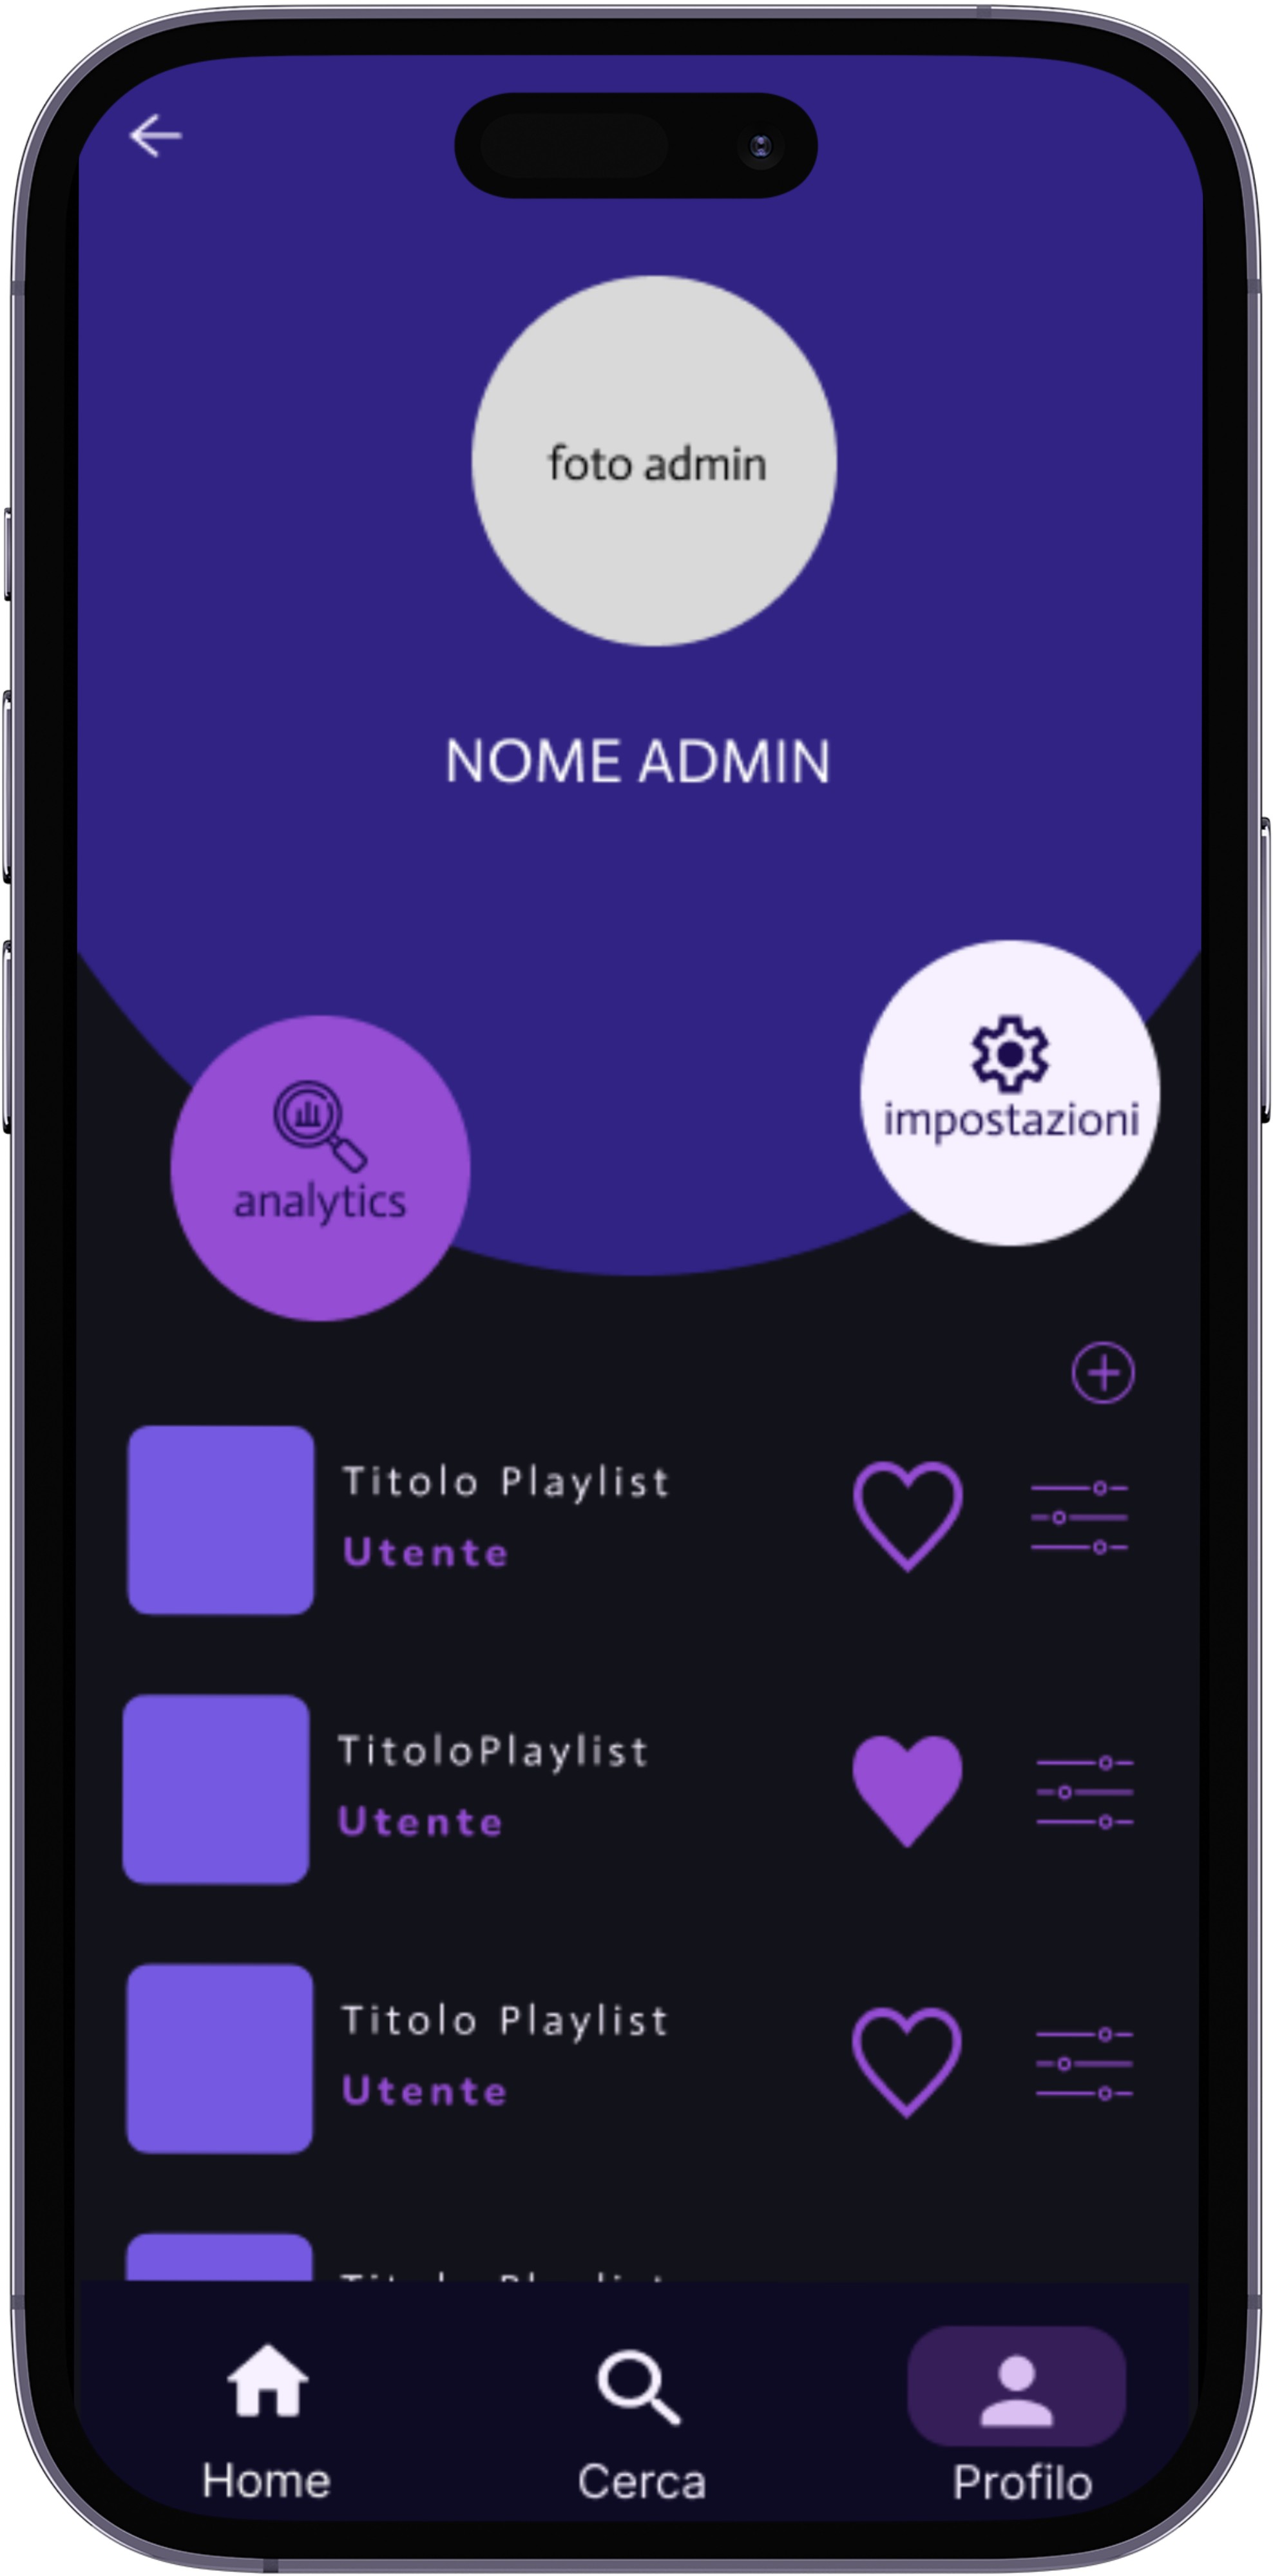
\includegraphics[width=\textwidth]{foto6}
				\end{minipage}
				\hfill
				\begin{minipage}{0.18\textwidth}
					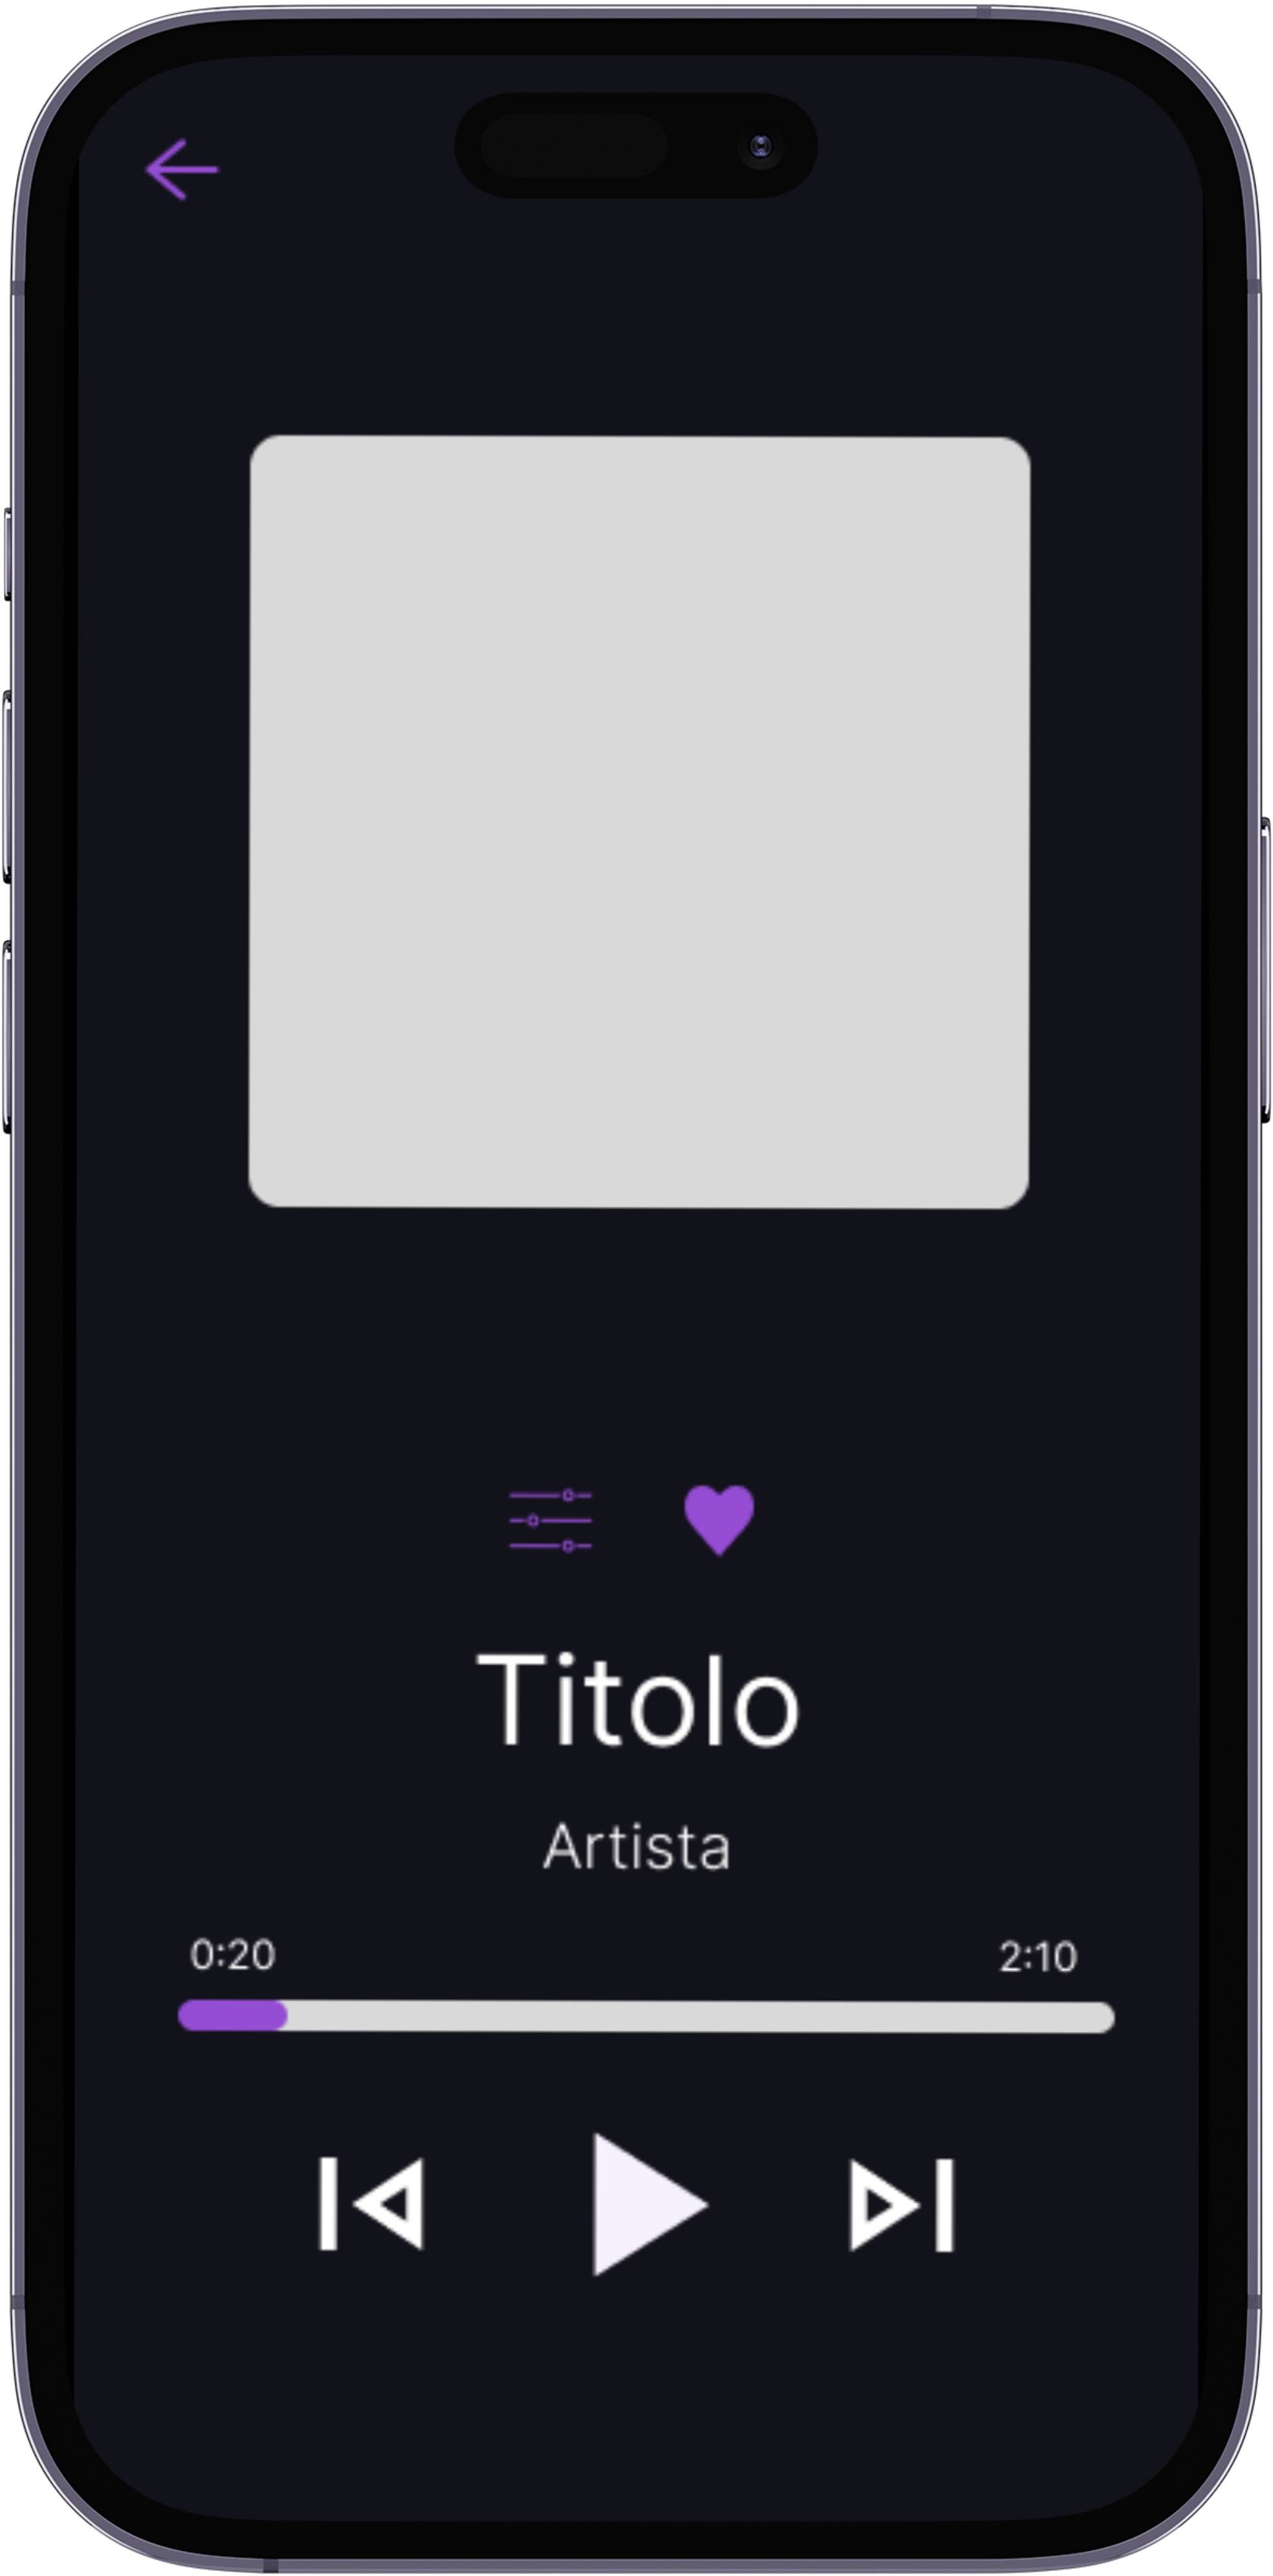
\includegraphics[width=\textwidth]{foto7}
				\end{minipage}
			\end{figure}
			\newpage
		Verranno mostrati, di seguito, i\textit{ mockup finali} di due metodi scelti ovvero: \textbf{visualizzazione analitiche} e \textbf{aggiunta traccia musicale ad una playlist}.
			\subsubsection{Mockup Visualizzazione analitiche}
			\textit{NOTA: è stato ritenuto opportuno riportare anche un caso d'errore.}
			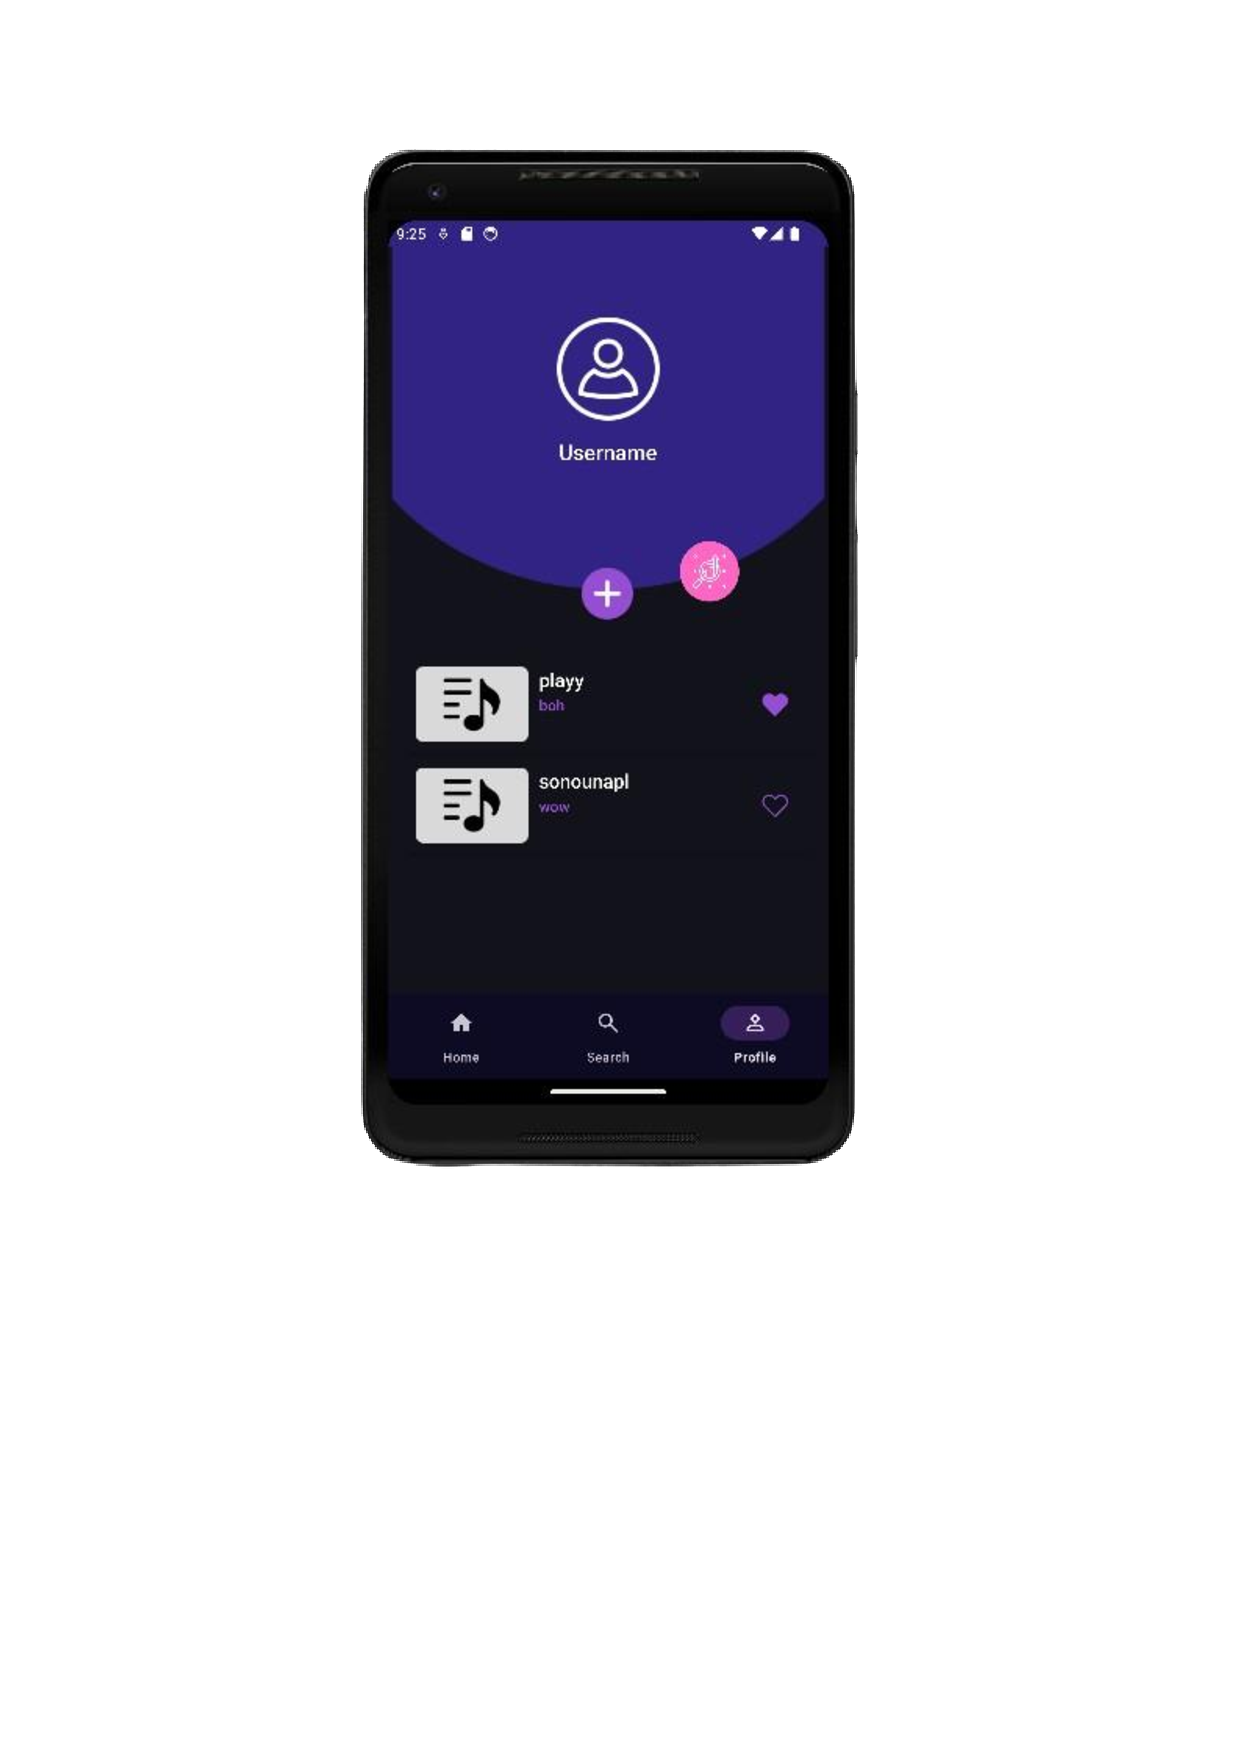
\includepdf[pages={1,2,3,4,5,6,7}]{mockupanalitiche}
			
			\subsubsection{Mockup Aggiunta traccia musicale ad una playlist}
			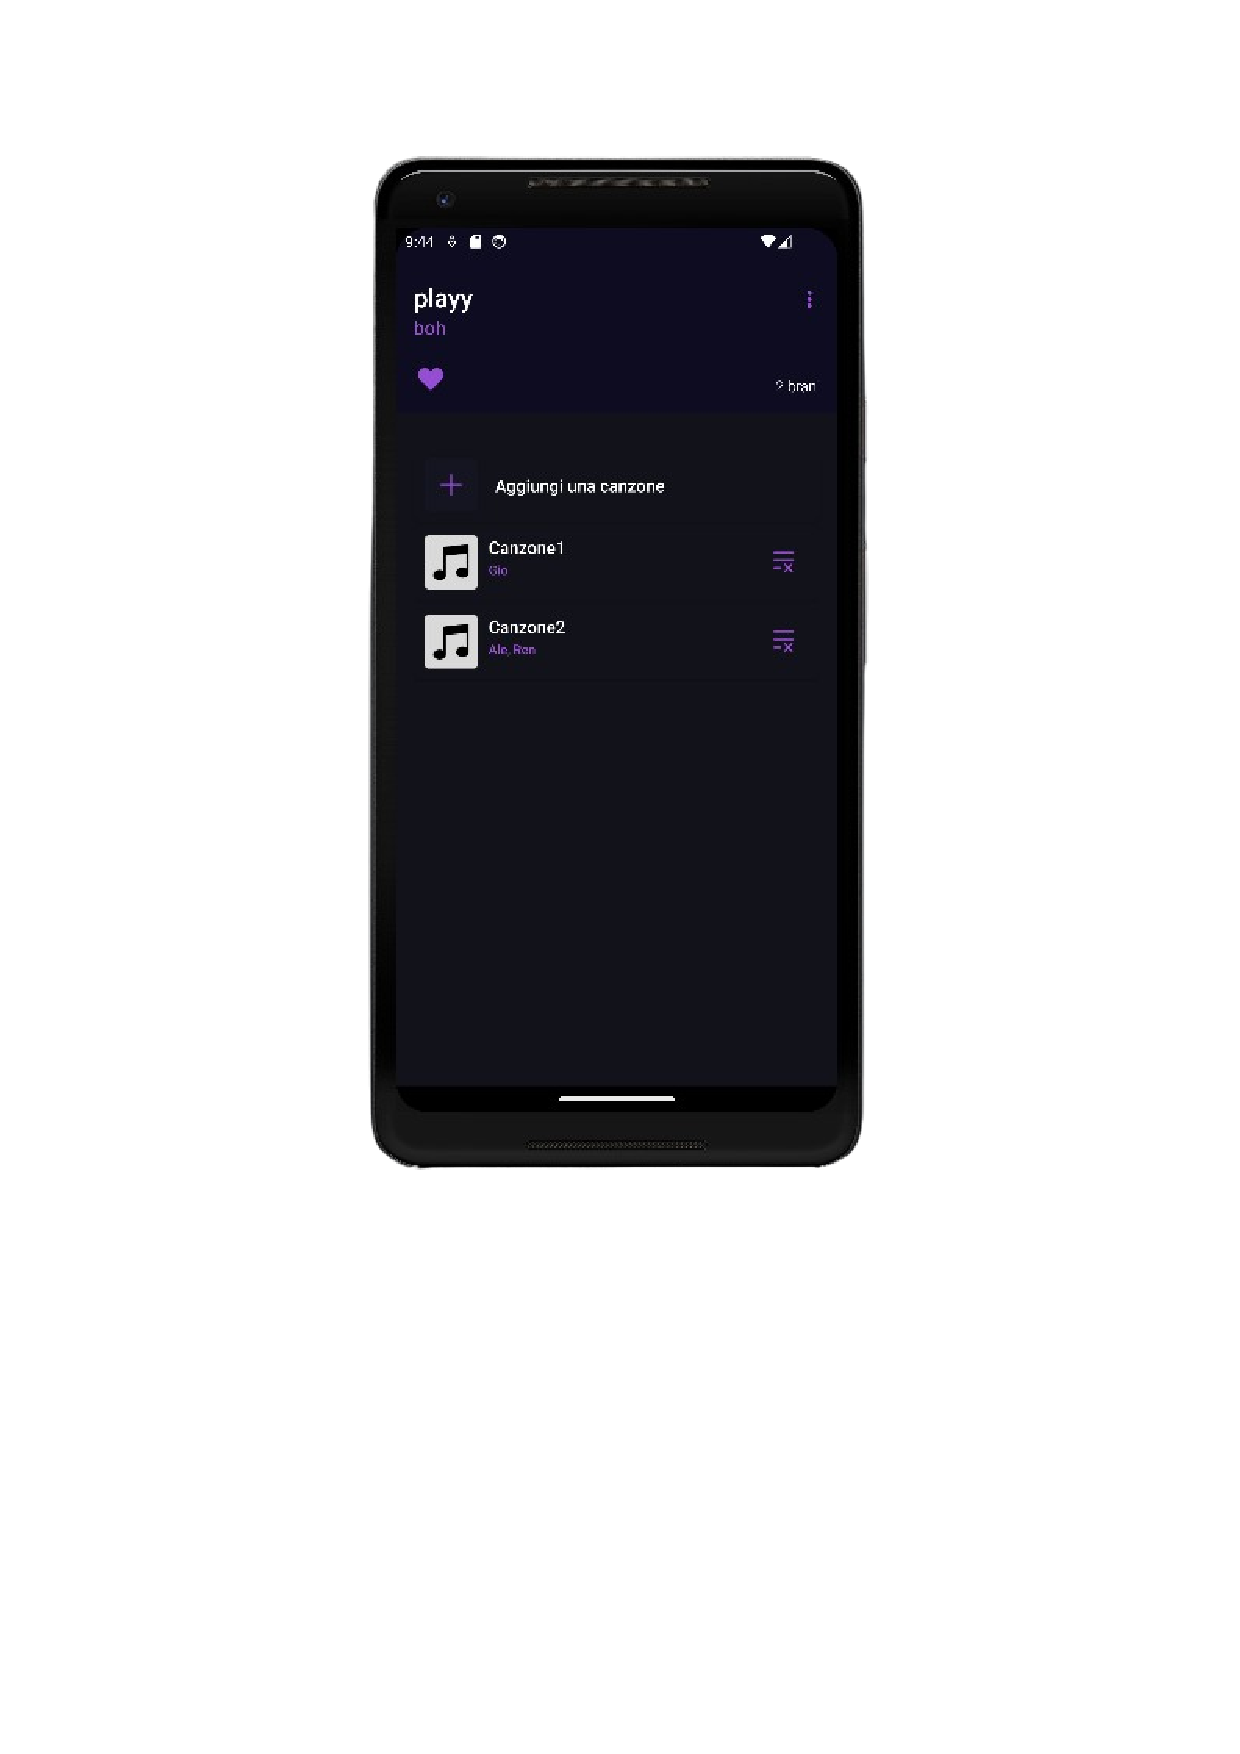
\includepdf[pages={1,2,3,4}]{mockupadd}
		\subsection{Presentazione dell'idea progettuale}
		\textbf{\textit{\textcolor{dark_purple}{Soundlab}}} nasce dall'esigenza di creare una piattaforma di streaming musicale che offra condizioni più vantaggiose per gli artisti, garantendo una remunerazione più equa e trasparente. Inoltre, si propone di migliorare significativamente l'esperienza dell'utente attraverso un'interfaccia più intuitiva e funzionalità innovative che permettano una maggiore personalizzazione dei contenuti.\\
		\textbf{\textit{\textcolor{dark_purple}{Soundlab}}} mira anche a differenziarsi con un catalogo musicale unico, promuovendo così una maggiore diversità musicale. Infine, una priorità fondamentale è garantire una maggiore tutela della privacy e sicurezza dei dati degli utenti, rispondendo alle crescenti preoccupazioni riguardo alla gestione delle informazioni personali.
		
			\subsubsection{Perchè abbiamo deciso di lavorare con la musica?}
			Al giorno d'oggi, lavorare con la musica o attraverso piattaforme ad essa dedicate offre numerosi vantaggi.\\ Innanzitutto, la \textbf{crescente diffusione della tecnologia} e \textbf{l'accesso a Internet} hanno reso la musica più facilmente fruibile a livello globale, ampliando il pubblico potenziale e le opportunità di mercato per artisti e imprenditori. \\Le piattaforme digitali consentono di \textbf{raggiungere rapidamente un vasto numero di ascoltatori}, superando le barriere geografiche e culturali.\\Inoltre, l'analisi dei dati e gli algoritmi di raccomandazione permettono di \textbf{comprendere meglio le preferenze degli utenti}, offrendo esperienze musicali personalizzate e aumentando l'engagement. Questo può tradursi in un maggior numero di stream, vendite e visibilità per gli artisti.\\
			Infine, lavorare con la musica attraverso piattaforme dedicate offre l'opportunità di \textbf{innovare costantemente}, sperimentando nuove tecnologie e format, come la realtà virtuale e aumentata, per arricchire l'esperienza dell'ascoltatore e mantenere un vantaggio competitivo in un settore in continua evoluzione.
			\subsubsection{Analisi delle funzionalità}
			\begin{itemize}
				\item \textbf{Un utente può registrarsi:} Gli utenti possono creare un account personale fornendo le informazioni necessarie, come email e password, per accedere alle funzionalità avanzate dell'app.
				\item \textbf{Un utente registrato può creare la propria playlist:} Dopo la registrazione, gli utenti possono creare playlist personalizzate, dando loro un nome e aggiungendo i brani preferiti.
				\item \textbf{Un utente registrato può eliminare una playlist:} Gli utenti hanno la possibilità di eliminare le playlist che non desiderano più mantenere.
				\item \textbf{Un utente registrato può aggiungere o rimuovere un brano dalla playlist:} Gli utenti possono modificare le loro playlist aggiungendo nuovi brani o rimuovendo quelli esistenti in base ai propri gusti.
				\item \textbf{Un utente registrato può ricercare un brano musicale e/o una playlist:} Gli utenti possono utilizzare la funzione di ricerca per trovare specifici brani musicali o playlist, facilitando l'accesso ai contenuti desiderati.
				\item \textbf{L'admin può visualizzare le analitiche dell'applicativo:} Gli amministratori hanno accesso alle statistiche e alle analitiche dell'app, come la fascia oraria in cui l'applicazione è più utilizzata, e altre metriche utili per monitorare e migliorare il servizio.
				\item \textbf{Un utente, sia esso admin o no, può modificare le impostazioni del proprio profilo:} Tutti gli utenti, inclusi gli amministratori, possono personalizzare le impostazioni del proprio profilo, come aggiornare le informazioni personali, modificare la password, modifcare l'email o cancellare il proprio profilo.
			\end{itemize}
			\subsubsection{Stato di sviluppo delle funzionalità}
			Nelle seguenti tabelle è stato rappresentato lo stato di sviluppo delle funzionalità ad oggi:
			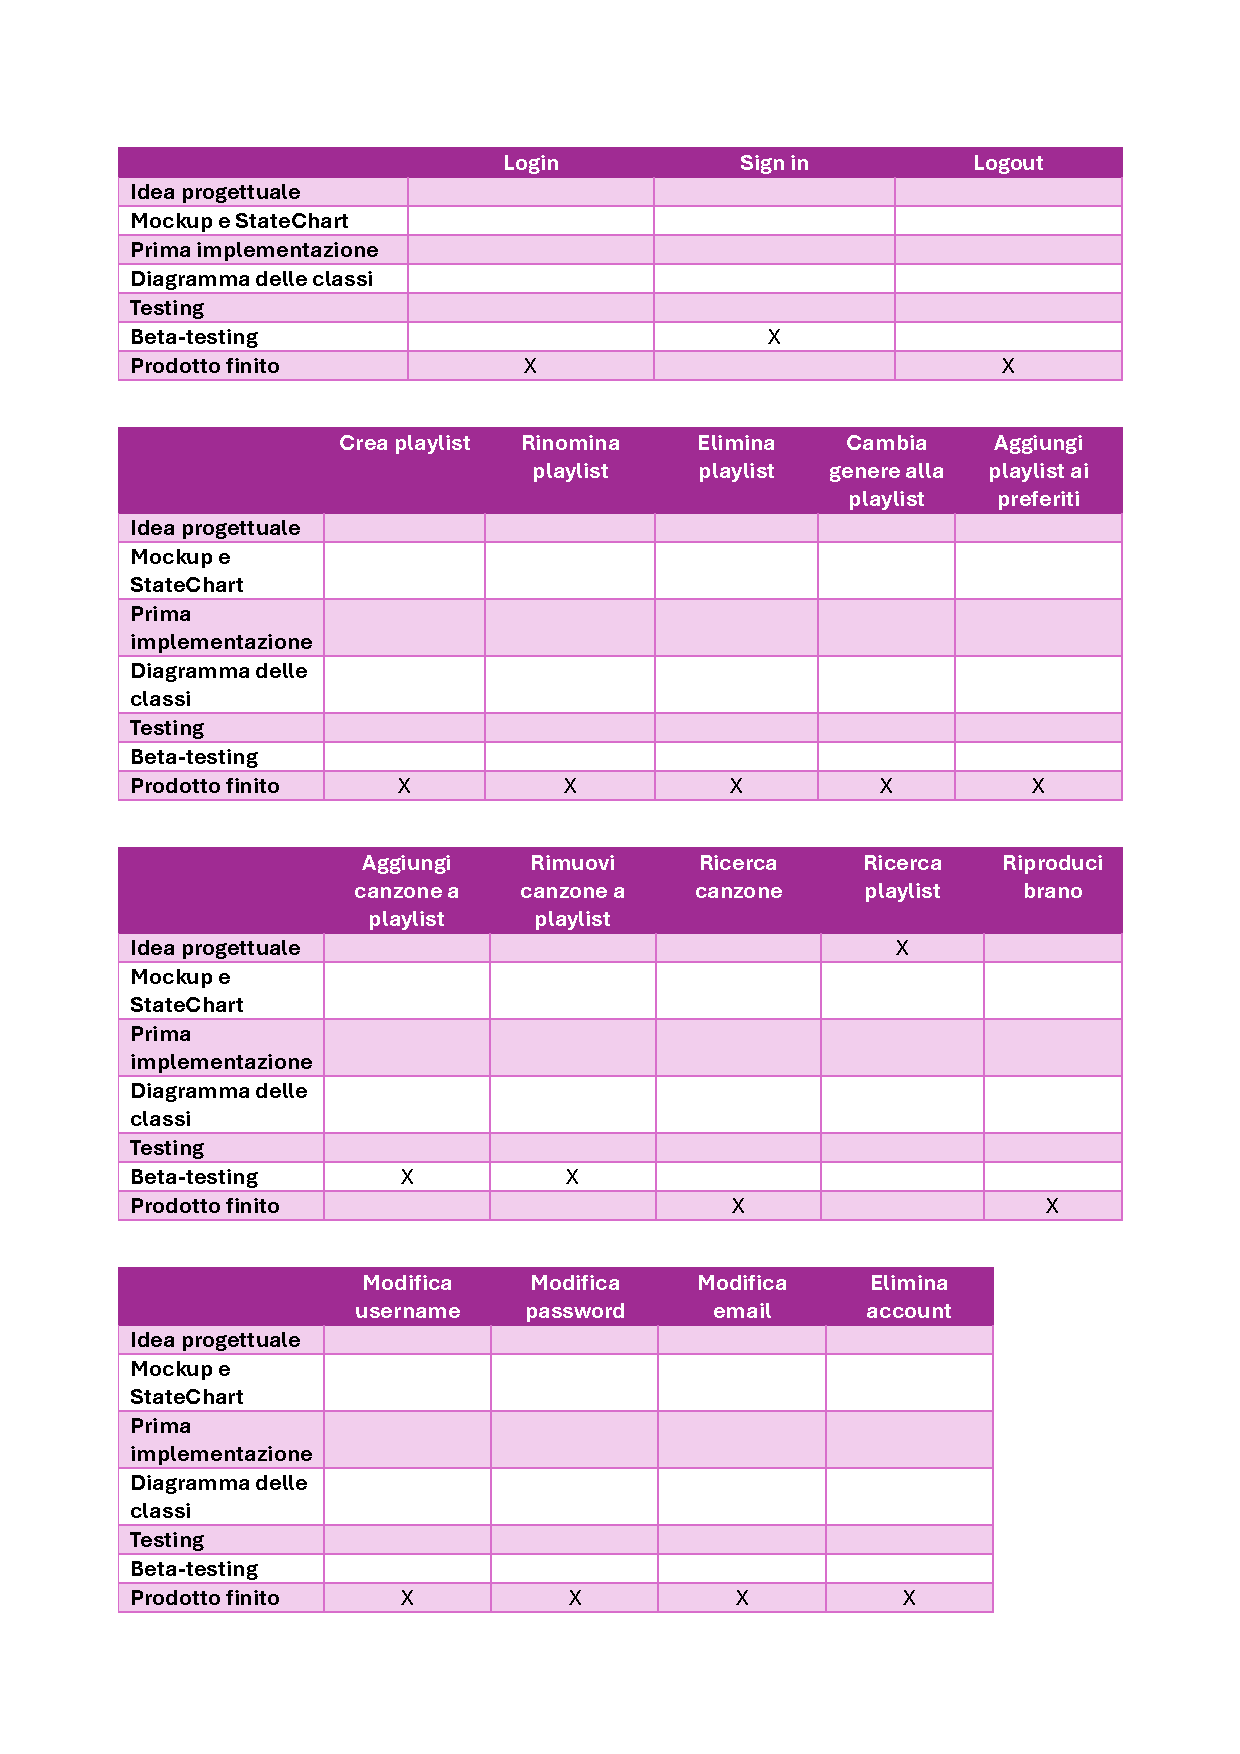
\includepdf[pages={1,2}]{tabelle.pdf}
		\subsection{Individuazione del target di utenti}
		Il target di utenti che si può definire da una prima (e relativa) analisi dei casi d’uso sono ovviamente:
		\begin{itemize}
			\item Utenti appassionati di musica
			\item Utenti che utilizzano piattaforme digitali
			\item Utenti interessati alla personalizzazione della loro esperienza musicale
		\end{itemize}
		Dal periodo della pandemia, l'utilizzo delle piattaforme di streaming musicale ha registrato un aumento significativo. Le persone hanno cercato nuovi modi per intrattenersi a casa, e lo streaming musicale è diventato una delle attività principali.\\
		Secondo i dati, nel 2021, la media settimanale di ascolto di musica era di 18,4 ore, rispetto alle 18 ore del 2019 e alle 17,8 ore del 2018 \textbf{(Gadget Advisor)}. Questo incremento è dovuto in gran parte alla crescita delle piattaforme di streaming musicale come Apple Music e Spotify, che hanno visto un aumento significativo nel numero di utenti e nel tempo di ascolto. Ad esempio, nel primo trimestre del 2023, sono stati superati un trilione di stream audio in soli tre mesi \textbf{(Gadget Advisor)}.\\
		Le statistiche mostrano che quasi il 40\% degli utenti di età compresa tra 35 e 64 anni ha utilizzato servizi di streaming musicale nell'ultimo mese, con una crescita particolarmente forte tra le generazioni più giovani, come i Millennial e la Generazione Z \textbf{(Comparitech)}.\\ Queste fasce d'età sono le più propense a sottoscrivere abbonamenti a servizi di streaming musicale per godere di un'esperienza senza pubblicità, la possibilità di scegliere la musica da ascoltare e l'accesso a vaste librerie di brani \textbf{(Comparitech)}.\\
		L'industria della musica in streaming ha visto una crescita continua negli ultimi anni. \\Nel 2022, il numero di brani ascoltati in streaming negli Stati Uniti ha raggiunto 1,3 trilioni, un aumento del 12,2\% rispetto all'anno precedente \textbf{(Comparitech)}. Inoltre, il mercato globale dello streaming musicale è cresciuto del 10,3\% nello stesso anno, segnando l'ottavo anno consecutivo di crescita per l'industria musicale \textbf{(Comparitech)}.\\
		Questi dati evidenziano come la pandemia abbia accelerato l'adozione e l'uso delle piattaforme di streaming musicale, che continuano a crescere grazie alla crescente domanda di contenuti musicali on-demand da parte di un pubblico sempre più ampio e diversificato.
			\subsubsection{Definizione delle Personas (3)}
			Il focus principale per individuare le user-personas è stato l'età.
			Per comodità, si è deciso di analizzare quattro fasce:
			\begin{itemize}
				\item \textbf{Gen Z:} età compresa tra i 10-23 anni
				\item \textbf{Millenials:} età compresa tra i 24-39 anni
				\item \textbf{oltre i 40 anni}
				\item \textbf{oltre i 60 anni}
			\end{itemize}
			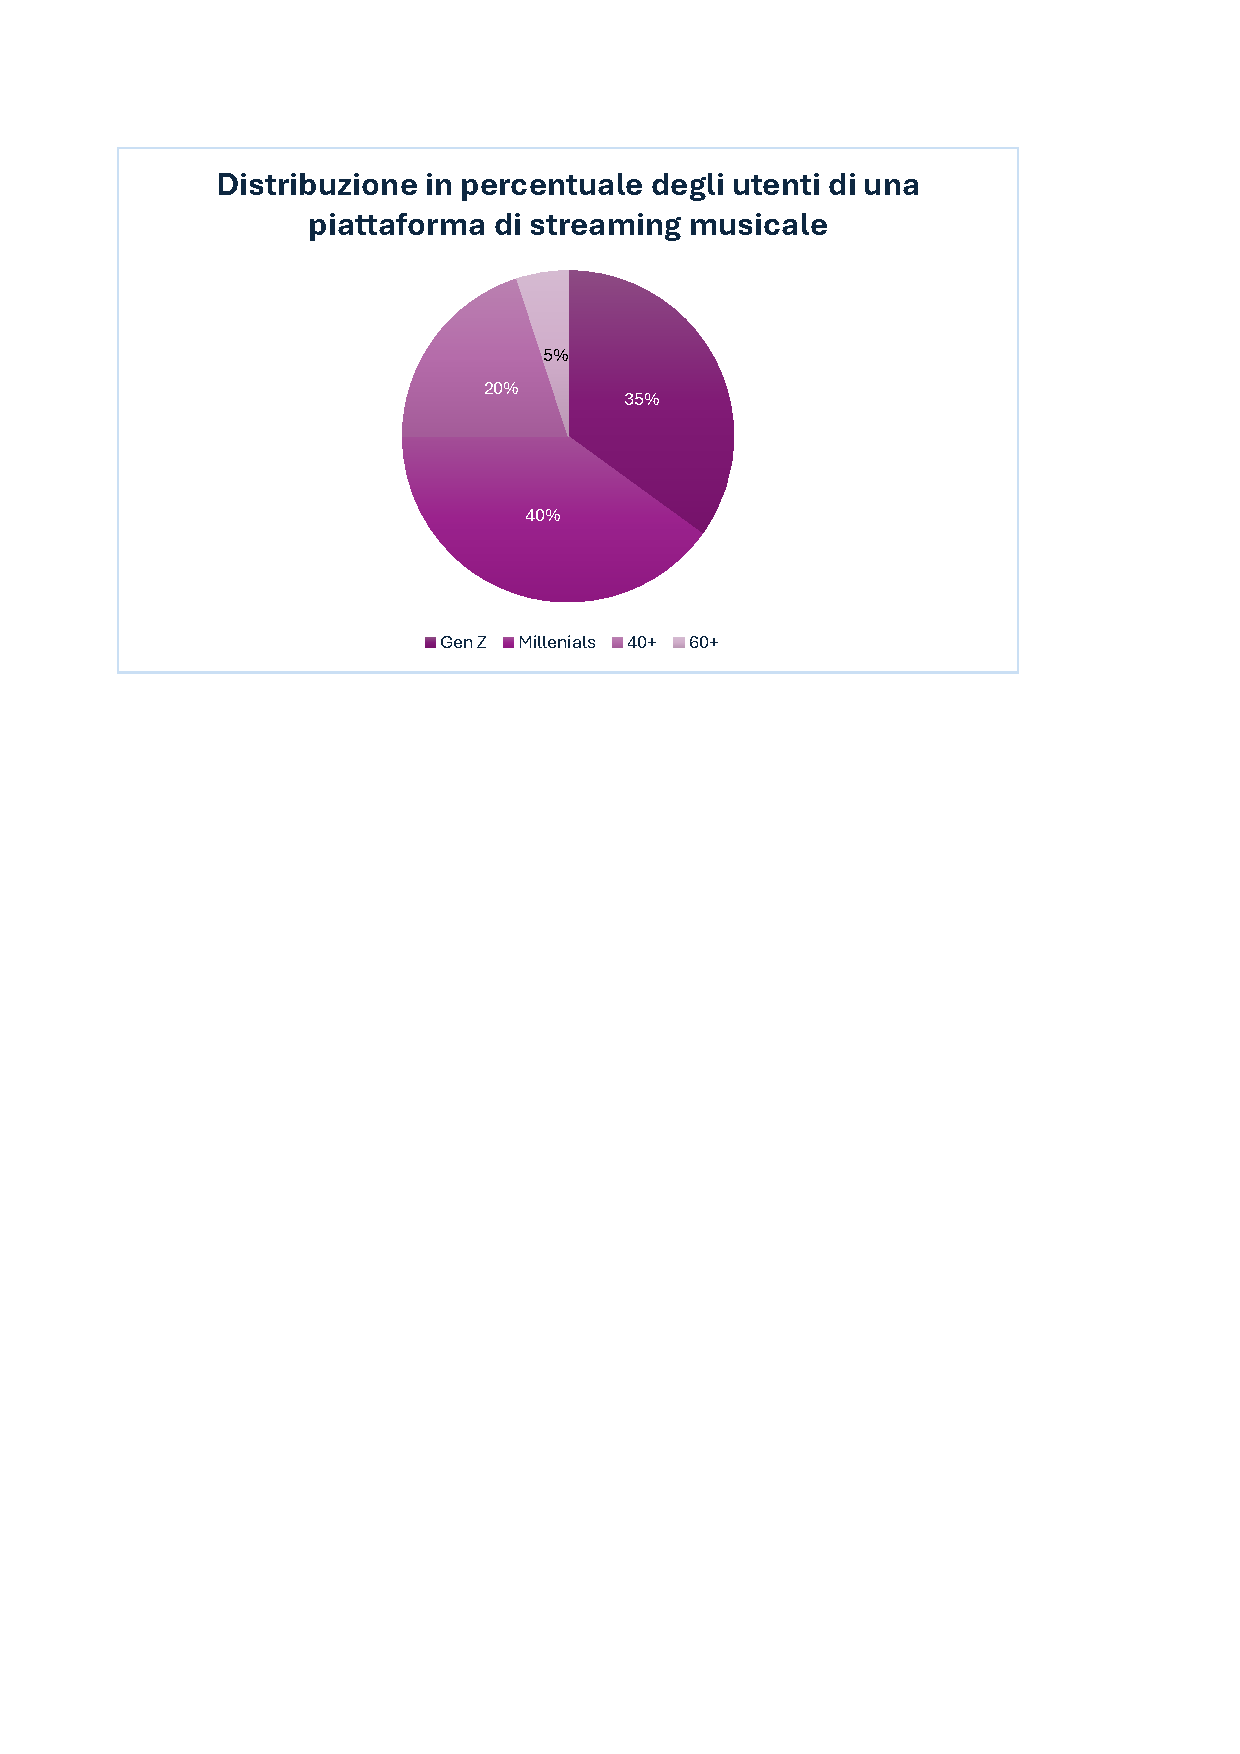
\includepdf[pages={1}]{dati.pdf}
		\subsection{Valutazione dell'usabilità a priori}
			\subsubsection{Tabelle di valutazione}
			\subsubsection{Tecnica utilizzata}
		\subsection{Glossario}
			\subsubsection{Termini}
			\subsubsection{Acronimi}
	\section{Modelli di dominio}
		\subsection{Classi, oggetti e relazioni di analisi}
			\subsubsection{Classi ed entità}
			\subsubsection{Class diagram delle funzionalità}
			\subsubsection{CLASS DIAGRAM DI TUTTE LE FUNZIONALITà}
		\subsection{Sequence diagram}
			\subsubsection{Funzionalità 1}
			\subsubsection{Funzionalità 2}
		\subsection{Activity diagram}
			\subsubsection{ACTIVITY DIAGRAM}
	\section{Design di sistema}
		\subsubsection{Analisi architetturale}
		\subsubsection{Descrizione architettura cloud}
		\subsubsection{Il server}
		\subsubsection{REST API}
		\subsubsection{Il client}
		\subsubsection{Supporti (RetroFit)}
		\subsubsection{Class Diagram di Design}
			\subsubsection{Diagrammi del punto USE CASE}
	\section{Codice sorgente sviluppato}
	\section{Codice xUnit}
		\subsubsection{Metodo 1}
		\subsubsection{Metodo 2}
		\subsubsection{Metodo 3}
		\subsubsection{Metodo 4}
	\section{Valutazione dell'usabilità sul campo}
		\subsubsection{Valutazione dell'applicativo}
		\subsubsection{Analisi delle performance}
		\subsubsection{Distribuzione ed accoglienza VALUTARE}
	\section{Conclusione (Riepilogo)}
		
\end{document}
